% Options for packages loaded elsewhere
\PassOptionsToPackage{unicode}{hyperref}
\PassOptionsToPackage{hyphens}{url}
%
\documentclass[
  ignorenonframetext,
]{beamer}
\usepackage{pgfpages}
\setbeamertemplate{caption}[numbered]
\setbeamertemplate{caption label separator}{: }
\setbeamercolor{caption name}{fg=normal text.fg}
\beamertemplatenavigationsymbolsempty
% Prevent slide breaks in the middle of a paragraph
\widowpenalties 1 10000
\raggedbottom
\setbeamertemplate{part page}{
  \centering
  \begin{beamercolorbox}[sep=16pt,center]{part title}
    \usebeamerfont{part title}\insertpart\par
  \end{beamercolorbox}
}
\setbeamertemplate{section page}{
  \centering
  \begin{beamercolorbox}[sep=12pt,center]{part title}
    \usebeamerfont{section title}\insertsection\par
  \end{beamercolorbox}
}
\setbeamertemplate{subsection page}{
  \centering
  \begin{beamercolorbox}[sep=8pt,center]{part title}
    \usebeamerfont{subsection title}\insertsubsection\par
  \end{beamercolorbox}
}
\AtBeginPart{
  \frame{\partpage}
}
\AtBeginSection{
  \ifbibliography
  \else
    \frame{\sectionpage}
  \fi
}
\AtBeginSubsection{
  \frame{\subsectionpage}
}
\usepackage{amsmath,amssymb}
\usepackage{lmodern}
\usepackage{iftex}
\ifPDFTeX
  \usepackage[T1]{fontenc}
  \usepackage[utf8]{inputenc}
  \usepackage{textcomp} % provide euro and other symbols
\else % if luatex or xetex
  \usepackage{unicode-math}
  \defaultfontfeatures{Scale=MatchLowercase}
  \defaultfontfeatures[\rmfamily]{Ligatures=TeX,Scale=1}
\fi
% Use upquote if available, for straight quotes in verbatim environments
\IfFileExists{upquote.sty}{\usepackage{upquote}}{}
\IfFileExists{microtype.sty}{% use microtype if available
  \usepackage[]{microtype}
  \UseMicrotypeSet[protrusion]{basicmath} % disable protrusion for tt fonts
}{}
\makeatletter
\@ifundefined{KOMAClassName}{% if non-KOMA class
  \IfFileExists{parskip.sty}{%
    \usepackage{parskip}
  }{% else
    \setlength{\parindent}{0pt}
    \setlength{\parskip}{6pt plus 2pt minus 1pt}}
}{% if KOMA class
  \KOMAoptions{parskip=half}}
\makeatother
\usepackage{xcolor}
\newif\ifbibliography
\usepackage{color}
\usepackage{fancyvrb}
\newcommand{\VerbBar}{|}
\newcommand{\VERB}{\Verb[commandchars=\\\{\}]}
\DefineVerbatimEnvironment{Highlighting}{Verbatim}{commandchars=\\\{\}}
% Add ',fontsize=\small' for more characters per line
\usepackage{framed}
\definecolor{shadecolor}{RGB}{248,248,248}
\newenvironment{Shaded}{\begin{snugshade}}{\end{snugshade}}
\newcommand{\AlertTok}[1]{\textcolor[rgb]{0.94,0.16,0.16}{#1}}
\newcommand{\AnnotationTok}[1]{\textcolor[rgb]{0.56,0.35,0.01}{\textbf{\textit{#1}}}}
\newcommand{\AttributeTok}[1]{\textcolor[rgb]{0.77,0.63,0.00}{#1}}
\newcommand{\BaseNTok}[1]{\textcolor[rgb]{0.00,0.00,0.81}{#1}}
\newcommand{\BuiltInTok}[1]{#1}
\newcommand{\CharTok}[1]{\textcolor[rgb]{0.31,0.60,0.02}{#1}}
\newcommand{\CommentTok}[1]{\textcolor[rgb]{0.56,0.35,0.01}{\textit{#1}}}
\newcommand{\CommentVarTok}[1]{\textcolor[rgb]{0.56,0.35,0.01}{\textbf{\textit{#1}}}}
\newcommand{\ConstantTok}[1]{\textcolor[rgb]{0.00,0.00,0.00}{#1}}
\newcommand{\ControlFlowTok}[1]{\textcolor[rgb]{0.13,0.29,0.53}{\textbf{#1}}}
\newcommand{\DataTypeTok}[1]{\textcolor[rgb]{0.13,0.29,0.53}{#1}}
\newcommand{\DecValTok}[1]{\textcolor[rgb]{0.00,0.00,0.81}{#1}}
\newcommand{\DocumentationTok}[1]{\textcolor[rgb]{0.56,0.35,0.01}{\textbf{\textit{#1}}}}
\newcommand{\ErrorTok}[1]{\textcolor[rgb]{0.64,0.00,0.00}{\textbf{#1}}}
\newcommand{\ExtensionTok}[1]{#1}
\newcommand{\FloatTok}[1]{\textcolor[rgb]{0.00,0.00,0.81}{#1}}
\newcommand{\FunctionTok}[1]{\textcolor[rgb]{0.00,0.00,0.00}{#1}}
\newcommand{\ImportTok}[1]{#1}
\newcommand{\InformationTok}[1]{\textcolor[rgb]{0.56,0.35,0.01}{\textbf{\textit{#1}}}}
\newcommand{\KeywordTok}[1]{\textcolor[rgb]{0.13,0.29,0.53}{\textbf{#1}}}
\newcommand{\NormalTok}[1]{#1}
\newcommand{\OperatorTok}[1]{\textcolor[rgb]{0.81,0.36,0.00}{\textbf{#1}}}
\newcommand{\OtherTok}[1]{\textcolor[rgb]{0.56,0.35,0.01}{#1}}
\newcommand{\PreprocessorTok}[1]{\textcolor[rgb]{0.56,0.35,0.01}{\textit{#1}}}
\newcommand{\RegionMarkerTok}[1]{#1}
\newcommand{\SpecialCharTok}[1]{\textcolor[rgb]{0.00,0.00,0.00}{#1}}
\newcommand{\SpecialStringTok}[1]{\textcolor[rgb]{0.31,0.60,0.02}{#1}}
\newcommand{\StringTok}[1]{\textcolor[rgb]{0.31,0.60,0.02}{#1}}
\newcommand{\VariableTok}[1]{\textcolor[rgb]{0.00,0.00,0.00}{#1}}
\newcommand{\VerbatimStringTok}[1]{\textcolor[rgb]{0.31,0.60,0.02}{#1}}
\newcommand{\WarningTok}[1]{\textcolor[rgb]{0.56,0.35,0.01}{\textbf{\textit{#1}}}}
\usepackage{longtable,booktabs,array}
\usepackage{calc} % for calculating minipage widths
\usepackage{caption}
% Make caption package work with longtable
\makeatletter
\def\fnum@table{\tablename~\thetable}
\makeatother
\usepackage{graphicx}
\makeatletter
\def\maxwidth{\ifdim\Gin@nat@width>\linewidth\linewidth\else\Gin@nat@width\fi}
\def\maxheight{\ifdim\Gin@nat@height>\textheight\textheight\else\Gin@nat@height\fi}
\makeatother
% Scale images if necessary, so that they will not overflow the page
% margins by default, and it is still possible to overwrite the defaults
% using explicit options in \includegraphics[width, height, ...]{}
\setkeys{Gin}{width=\maxwidth,height=\maxheight,keepaspectratio}
% Set default figure placement to htbp
\makeatletter
\def\fps@figure{htbp}
\makeatother
\setlength{\emergencystretch}{3em} % prevent overfull lines
\providecommand{\tightlist}{%
  \setlength{\itemsep}{0pt}\setlength{\parskip}{0pt}}
\setcounter{secnumdepth}{-\maxdimen} % remove section numbering
\usepackage{bbm}
\ifLuaTeX
  \usepackage{selnolig}  % disable illegal ligatures
\fi
\IfFileExists{bookmark.sty}{\usepackage{bookmark}}{\usepackage{hyperref}}
\IfFileExists{xurl.sty}{\usepackage{xurl}}{} % add URL line breaks if available
\urlstyle{same} % disable monospaced font for URLs
\hypersetup{
  pdftitle={MQE: Economic Inference from Data: Odds and Ends},
  pdfauthor={Claire Duquennois},
  hidelinks,
  pdfcreator={LaTeX via pandoc}}

\title{MQE: Economic Inference from Data:\\
Odds and Ends}
\author{Claire Duquennois}
\date{2020}

\begin{document}
\frame{\titlepage}

\begin{frame}{Odds and Ends}
\protect\hypertarget{odds-and-ends}{}
\begin{itemize}
\item
  Regression Interpretation

  \begin{itemize}
  \tightlist
  \item
    Binairy Dependent Variables
  \end{itemize}
\item
  Non-Standard Standard Errors
\item
  Confidence intervals for predictions
\item
  Spatial Data
\end{itemize}
\end{frame}

\hypertarget{regression-interpretation-and-variable-transformations}{%
\section{Regression Interpretation and Variable
Transformations}\label{regression-interpretation-and-variable-transformations}}

\begin{frame}{Regression Interpretation}
\protect\hypertarget{regression-interpretation}{}
You must be able to interpret a regression correctly.

3 elements you want to touch upon (the three S'):

\begin{enumerate}
[1)]
\item
  \textbf{Sign}- is the coefficient you are discussing positive or
  negative? Does the sign of the coefficient match your priors or is it
  surprising?
\item
  \textbf{Size}- What is the magnitude of the coefficient? Is the effect
  of \(x\) on \(y\) economically meaningful or not? Make your
  interpretation informative to your audience,by being precise.
\item
  \textbf{Significance}- Is the estimate statistically significant? Can
  we reject that the true coefficient is equal to zero? With what
  confidence level?
\end{enumerate}
\end{frame}

\begin{frame}{Regression Interpretation}
\protect\hypertarget{regression-interpretation-1}{}
While it is not incorrect to say the that a one unit increase in \(x\)
leads to a \(\beta\) unit change in \(y\), you will generally want to be
more precise:

\begin{itemize}
\item
  specify the units of measurement
\item
  interpret the coefficients appropriately:

  \begin{itemize}
  \item
    if the regression used a logged variable, a binairy dependent
    variable, a standardized variable\ldots{}
  \item
    it may be useful to scale the values into more intuitive units.
  \end{itemize}
\item
  If the regression features a polynomial discuss the difference in the
  magnitude of the marginal effects at different key values.
\item
  If the regression features interaction terms, interpret the
  implications for different types of observations
\item
  it is often useful to compare the coefficient to the mean and sd of
  the dependent variable to gauge magnitudes
\end{itemize}
\end{frame}

\begin{frame}{Regression Interpretation}
\protect\hypertarget{regression-interpretation-2}{}
\begin{itemize}
\item
  Scaling
\item
  Standardizing
\item
  Regressions in Logs
\item
  Quadratics
\item
  Interactions with Continuous Variables
\item
  Binairy Dependent variables

  \begin{itemize}
  \item
    Linear probability Models
  \item
    Logits
  \end{itemize}
\end{itemize}
\end{frame}

\hypertarget{scaling}{%
\section{Scaling}\label{scaling}}

\begin{frame}[fragile]{Scaling}
\protect\hypertarget{scaling-1}{}
Units of measurement in the data are not always intuitive.

Suppose I am interested in the following regression: \[
sleep=\beta_0+\beta_1totwork+\beta_2educ+u
\] Using the \texttt{sleep75} data that is part of the
\texttt{wooldrige} package:

\tiny

\begin{Shaded}
\begin{Highlighting}[]
\NormalTok{regsleep1}\OtherTok{\textless{}{-}}\FunctionTok{lm}\NormalTok{(sleep}\SpecialCharTok{\textasciitilde{}}\NormalTok{totwrk}\SpecialCharTok{+}\NormalTok{educ, sleep75)}
\FunctionTok{summary}\NormalTok{(regsleep1)}
\end{Highlighting}
\end{Shaded}

\begin{verbatim}
## 
## Call:
## lm(formula = sleep ~ totwrk + educ, data = sleep75)
## 
## Residuals:
##      Min       1Q   Median       3Q      Max 
## -2441.18  -235.18    18.13   259.76  1329.94 
## 
## Coefficients:
##               Estimate Std. Error t value Pr(>|t|)    
## (Intercept) 3756.21512   81.28699  46.209   <2e-16 ***
## totwrk        -0.14945    0.01669  -8.952   <2e-16 ***
## educ         -13.50385    5.68001  -2.377   0.0177 *  
## ---
## Signif. codes:  0 '***' 0.001 '**' 0.01 '*' 0.05 '.' 0.1 ' ' 1
## 
## Residual standard error: 419.8 on 703 degrees of freedom
## Multiple R-squared:  0.1104, Adjusted R-squared:  0.1079 
## F-statistic: 43.64 on 2 and 703 DF,  p-value: < 2.2e-16
\end{verbatim}
\end{frame}

\begin{frame}{Scaling}
\protect\hypertarget{scaling-2}{}
What do these coefficients mean?

You need to know the units of measurement for each of the variables:

\begin{itemize}
\item
  \(educ\) is measured in years of education
\item
  \(sleep\) and \(totwrk\) are measured in minutes per week.
\end{itemize}

\textbf{one additional year of education is associated with 13.5 fewer
minutes of sleep per week}.

\(\Rightarrow\) probably not the most intuitive interpretation
\end{frame}

\begin{frame}{Scaling the dependent variable}
\protect\hypertarget{scaling-the-dependent-variable}{}
One way, adjustment in interpretation: \(13.5\) min per week
\(=\frac{13.5}{60}=0.23\approx 1/4\) hour per week.

Rewrite interpretations in terms of hours by dividing the old
coefficients by 60: \[
\frac{\hat{\beta}_0}{60};\frac{\hat{\beta}_1}{60};\frac{\hat{\beta}_2}{60}. 
\]
\end{frame}

\begin{frame}[fragile]{Scaling the dependent variable}
\protect\hypertarget{scaling-the-dependent-variable-1}{}
Alternatively, run the regression after having scaled our \(sleep\)
variable in terms of hours: \tiny

\begin{Shaded}
\begin{Highlighting}[]
\NormalTok{sleep75}\SpecialCharTok{$}\NormalTok{sleephrs}\OtherTok{\textless{}{-}}\NormalTok{sleep75}\SpecialCharTok{$}\NormalTok{sleep}\SpecialCharTok{/}\DecValTok{60}

\NormalTok{regsleep2}\OtherTok{\textless{}{-}}\FunctionTok{lm}\NormalTok{(sleephrs}\SpecialCharTok{\textasciitilde{}}\NormalTok{totwrk}\SpecialCharTok{+}\NormalTok{educ, sleep75)}
\FunctionTok{summary}\NormalTok{(regsleep2)}
\end{Highlighting}
\end{Shaded}

\begin{verbatim}
## 
## Call:
## lm(formula = sleephrs ~ totwrk + educ, data = sleep75)
## 
## Residuals:
##     Min      1Q  Median      3Q     Max 
## -40.686  -3.920   0.302   4.329  22.166 
## 
## Coefficients:
##               Estimate Std. Error t value Pr(>|t|)    
## (Intercept) 62.6035854  1.3547832  46.209   <2e-16 ***
## totwrk      -0.0024909  0.0002782  -8.952   <2e-16 ***
## educ        -0.2250641  0.0946669  -2.377   0.0177 *  
## ---
## Signif. codes:  0 '***' 0.001 '**' 0.01 '*' 0.05 '.' 0.1 ' ' 1
## 
## Residual standard error: 6.996 on 703 degrees of freedom
## Multiple R-squared:  0.1104, Adjusted R-squared:  0.1079 
## F-statistic: 43.64 on 2 and 703 DF,  p-value: < 2.2e-16
\end{verbatim}
\end{frame}

\begin{frame}{Scaling the dependent variable}
\protect\hypertarget{scaling-the-dependent-variable-2}{}
If we re-scale the dependent variable \(y\) by a constant \(c\), then
the equation we estimate becomes

\[
\begin{aligned}
\tilde{y}&=\tilde{\beta}_0+\tilde{\beta}_1x_1+...+\tilde{\beta}_kx_k+u\\
cy&=c\beta_0+c\beta_1x_1+c\beta_2x2+...+c\beta_kx_k+u.
\end{aligned}
\] In the example above, \(c=\frac{1}{60}\), so the new
\(\hat{\beta}\)'s will be divided by 60 too.

Nothing else about the regression changes (\(R^2\), t-stats, p-values).
\end{frame}

\begin{frame}[fragile]{Scaling the independent variable}
\protect\hypertarget{scaling-the-independent-variable}{}
1 minute increase in total work per week predicts a decrease in sleep of
0.0025 hours per week.

\(\Rightarrow\) one hour increase in total work predicts a
60*(0.0025)=0.15 hour decrease in sleep per week.

Scale the variable in R prior to running the regression: \tiny

\begin{Shaded}
\begin{Highlighting}[]
\NormalTok{sleep75}\SpecialCharTok{$}\NormalTok{totwrkhrs}\OtherTok{\textless{}{-}}\NormalTok{sleep75}\SpecialCharTok{$}\NormalTok{totwrk}\SpecialCharTok{/}\DecValTok{60}

\NormalTok{regsleep3}\OtherTok{\textless{}{-}}\FunctionTok{lm}\NormalTok{(sleephrs}\SpecialCharTok{\textasciitilde{}}\NormalTok{totwrkhrs}\SpecialCharTok{+}\NormalTok{educ, sleep75)}
\FunctionTok{summary}\NormalTok{(regsleep3)}
\end{Highlighting}
\end{Shaded}

\begin{verbatim}
## 
## Call:
## lm(formula = sleephrs ~ totwrkhrs + educ, data = sleep75)
## 
## Residuals:
##     Min      1Q  Median      3Q     Max 
## -40.686  -3.920   0.302   4.329  22.166 
## 
## Coefficients:
##             Estimate Std. Error t value Pr(>|t|)    
## (Intercept) 62.60359    1.35478  46.209   <2e-16 ***
## totwrkhrs   -0.14945    0.01669  -8.952   <2e-16 ***
## educ        -0.22506    0.09467  -2.377   0.0177 *  
## ---
## Signif. codes:  0 '***' 0.001 '**' 0.01 '*' 0.05 '.' 0.1 ' ' 1
## 
## Residual standard error: 6.996 on 703 degrees of freedom
## Multiple R-squared:  0.1104, Adjusted R-squared:  0.1079 
## F-statistic: 43.64 on 2 and 703 DF,  p-value: < 2.2e-16
\end{verbatim}
\end{frame}

\begin{frame}{Scaling the independent variable}
\protect\hypertarget{scaling-the-independent-variable-1}{}
The other coefficients will be unchanged.

The coefficient on the scaled variable will adjust accordingly.

In general, if we scale \(x\) by \(c\), the equation becomes:

\[
\begin{aligned}
y&= \beta_0+\tilde{\beta}_1\tilde{x}_1+...+\beta_kx_k+u\\
&= \beta_0+\frac{\tilde{\beta}_1}{c}(c\tilde{x}_1)+...+\beta_kx_k+u.
\end{aligned}
\]
\end{frame}

\hypertarget{standardizing}{%
\section{Standardizing}\label{standardizing}}

\begin{frame}{Standardizing}
\protect\hypertarget{standardizing-1}{}
Standardizing variables eliminates the units:

\begin{itemize}
\item
  makes it possible to compare the magnitude of estimates across
  independent variables.
\item
  makes interpretation easier if you have variables with weird arbitrary
  units that are unfamiliar to people.
\end{itemize}
\end{frame}

\begin{frame}{Standardizing}
\protect\hypertarget{standardizing-2}{}
Suppose we have a regression with two variables, \(x_1\) and \(x_2\):

\[
y=\hat{\beta}_0+\hat{\beta}_1 x_1 +\hat{\beta}_2x_2+\hat{u}
\]

A linear regression must go through the point of averages:

\begin{itemize}
\tightlist
\item
  if we plugged in \(\bar{x}_1\) and \(\bar{x}_2\), we would predict
  \(\bar{y}\):
\end{itemize}

\[
\bar{y}=\hat{\beta}_0+\hat{\beta}_1\bar{x}_1 +\hat{\beta}_2\bar{x}_2
\]
\end{frame}

\begin{frame}{Standardizing}
\protect\hypertarget{standardizing-3}{}
We can subtract the second equation from the first to get: \[
\begin{aligned}
\hat{y}-\bar{y}&=(\hat{\beta}_0+\hat{\beta}_1 x_1 +\hat{\beta}_2
x_2+\hat{u})-(\hat{\beta}_0+\hat{\beta}_1\bar{x}_1 +\hat{\beta}_2\bar{x}_2)\\
&=\hat{\beta}_1( x_1-\bar{x}_1) +\hat{\beta}_2(
x_2-\bar{x}_2)+\hat{u}
\end{aligned}
\] Dividing both sides of this equation by the standard deviation of
\(y\), \(\sigma_y\) and multiplying each independent variable by
\(1=\frac{\sigma_x}{\sigma_x}\), we can get the regression into standard
units:

\[
(\frac{y-\bar{y}}{\hat{\sigma}_y})=\frac{\hat{\sigma}_{x_1}}{\hat{\sigma}_y}\hat{\beta}_1(\frac{x_1-\bar{x}_1}{\hat{\sigma}_{x_1}})+\frac{\hat{\sigma}_{x_2}}{\hat{\sigma}_y}\hat{\beta}_2(\frac{x_2-\bar{x}_2}{\hat{\sigma}_{x_2}})+\frac{\hat{u}}{\hat{\sigma}_y}
\]
\end{frame}

\begin{frame}{Standardizing}
\protect\hypertarget{standardizing-4}{}
Controlling for \(x_2\) a \textbf{one standard deviation} increase in
\(x_1\) leads to a
\(\frac{\hat{\sigma}_{x_1}}{\hat{\sigma}_y}\hat{\beta}_1\)
\textbf{standard deviation} increase in the predicted \(y\).

This is the standardized coefficient or ``beta'' coefficient.

It is also possible to only standardize some variables ( you will need
an intercept in this case).
\end{frame}

\begin{frame}[fragile]{Standardizing}
\protect\hypertarget{standardizing-5}{}
In R, we can get these coefficients by using the \texttt{scale()}
command in \texttt{R}.

We use the bwght2 dataset to look at how parent ages correlate with
birth weights. (Note: birth weights here will be measured in grams).

I estimate four different regressions of the type \[
birthweight_i=\beta_0+\beta_1 motherage_i+\beta_2 fatherage_i+\epsilon_i
\]

scaling either the dependent and/or independent variables.
\end{frame}

\begin{frame}[fragile]{Standardizing}
\protect\hypertarget{standardizing-6}{}
\tiny

\begin{Shaded}
\begin{Highlighting}[]
\NormalTok{reg1}\OtherTok{\textless{}{-}}\FunctionTok{lm}\NormalTok{(bwght}\SpecialCharTok{\textasciitilde{}}\NormalTok{mage}\SpecialCharTok{+}\NormalTok{fage, bwght2)}
\NormalTok{reg2}\OtherTok{\textless{}{-}}\FunctionTok{lm}\NormalTok{(}\FunctionTok{scale}\NormalTok{(bwght)}\SpecialCharTok{\textasciitilde{}}\FunctionTok{scale}\NormalTok{(mage)}\SpecialCharTok{+}\FunctionTok{scale}\NormalTok{(fage), bwght2)}
\NormalTok{reg3}\OtherTok{\textless{}{-}}\FunctionTok{lm}\NormalTok{(}\FunctionTok{scale}\NormalTok{(bwght)}\SpecialCharTok{\textasciitilde{}}\NormalTok{mage}\SpecialCharTok{+}\NormalTok{fage, bwght2)}
\NormalTok{reg4}\OtherTok{\textless{}{-}}\FunctionTok{lm}\NormalTok{(bwght}\SpecialCharTok{\textasciitilde{}}\FunctionTok{scale}\NormalTok{(mage)}\SpecialCharTok{+}\FunctionTok{scale}\NormalTok{(fage), bwght2)}

\NormalTok{meandep1}\OtherTok{\textless{}{-}}\FunctionTok{round}\NormalTok{(}\FunctionTok{mean}\NormalTok{(bwght2}\SpecialCharTok{$}\NormalTok{bwght),}\DecValTok{2}\NormalTok{)}
\NormalTok{meandep2}\OtherTok{\textless{}{-}}\FunctionTok{round}\NormalTok{(}\FunctionTok{mean}\NormalTok{(}\FunctionTok{scale}\NormalTok{(bwght2}\SpecialCharTok{$}\NormalTok{bwght)),}\DecValTok{2}\NormalTok{)}
\NormalTok{sddep1}\OtherTok{\textless{}{-}}\FunctionTok{round}\NormalTok{(}\FunctionTok{sd}\NormalTok{(bwght2}\SpecialCharTok{$}\NormalTok{bwght),}\DecValTok{2}\NormalTok{)}
\NormalTok{sddep2}\OtherTok{\textless{}{-}}\FunctionTok{round}\NormalTok{(}\FunctionTok{sd}\NormalTok{(}\FunctionTok{scale}\NormalTok{(bwght2}\SpecialCharTok{$}\NormalTok{bwght)),}\DecValTok{2}\NormalTok{)}
\end{Highlighting}
\end{Shaded}
\end{frame}

\begin{frame}[fragile]{Standardizing}
\protect\hypertarget{standardizing-7}{}
\tiny

\begin{Shaded}
\begin{Highlighting}[]
\FunctionTok{stargazer}\NormalTok{(reg1,reg2, reg3, reg4, }\AttributeTok{type =} \StringTok{"latex"}\NormalTok{ , }\AttributeTok{header=}\ConstantTok{FALSE}\NormalTok{,}\AttributeTok{omit.stat =} \StringTok{"all"}\NormalTok{,}
          \AttributeTok{add.lines=}\FunctionTok{list}\NormalTok{(}\FunctionTok{c}\NormalTok{(}\StringTok{"Mean"}\NormalTok{,meandep1,meandep2, meandep2, meandep1 ),}
                         \FunctionTok{c}\NormalTok{(}\StringTok{"SD"}\NormalTok{,sddep1,sddep2, sddep2, sddep1 )))}
\end{Highlighting}
\end{Shaded}

\begin{table}[!htbp] \centering 
  \caption{} 
  \label{} 
\begin{tabular}{@{\extracolsep{5pt}}lcccc} 
\\[-1.8ex]\hline 
\hline \\[-1.8ex] 
 & \multicolumn{4}{c}{\textit{Dependent variable:}} \\ 
\cline{2-5} 
\\[-1.8ex] & bwght & \multicolumn{2}{c}{scale(bwght)} & bwght \\ 
\\[-1.8ex] & (1) & (2) & (3) & (4)\\ 
\hline \\[-1.8ex] 
 mage & $-$3.992 &  & $-$0.007 &  \\ 
  & (3.943) &  & (0.007) &  \\ 
  & & & & \\ 
 fage & 9.313$^{***}$ &  & 0.016$^{***}$ &  \\ 
  & (3.291) &  & (0.006) &  \\ 
  & & & & \\ 
 scale(mage) &  & $-$0.033 &  & $-$19.044 \\ 
  &  & (0.033) &  & (18.812) \\ 
  & & & & \\ 
 scale(fage) &  & 0.092$^{***}$ &  & 53.205$^{***}$ \\ 
  &  & (0.033) &  & (18.803) \\ 
  & & & & \\ 
 Constant & 3,221.030$^{***}$ & $-$0.001 & $-$0.312$^{**}$ & 3,400.304$^{***}$ \\ 
  & (87.703) & (0.023) & (0.152) & (13.448) \\ 
  & & & & \\ 
\hline \\[-1.8ex] 
Mean & 3401.12 & 0 & 0 & 3401.12 \\ 
SD & 576.54 & 1 & 1 & 576.54 \\ 
\hline 
\hline \\[-1.8ex] 
\textit{Note:}  & \multicolumn{4}{r}{$^{*}$p$<$0.1; $^{**}$p$<$0.05; $^{***}$p$<$0.01} \\ 
\end{tabular} 
\end{table}
\end{frame}

\begin{frame}{Standardizing}
\protect\hypertarget{standardizing-8}{}
\tiny

Interpreting column 1:

\begin{itemize}
\item
  A mother that is \textbf{a year} older predicts a birthweight that is
  3.992 \textbf{grams} less (not significant).
\item
  A father that is \textbf{a year} older predicts a birthweight that is
  9.313 \textbf{grams} more (significant).
\end{itemize}

Interpreting column 2:

\begin{itemize}
\item
  A mother whose age is \textbf{one standard deviation higher} predicts
  a birthweight that is 0.033 \textbf{standard deviations} lower (not
  significant).
\item
  A father whose age is \textbf{one standard deviation higher} predicts
  a birthweight that is 0.092 \textbf{standard deviations} higher
  (significant).
\end{itemize}

Interpreting column 3:

\begin{itemize}
\item
  A mother that is \textbf{a year} older predicts a birthweight that is
  0.007 \textbf{standard deviations} lower (not significant).
\item
  A father that is \textbf{a year} older predict a birthweight that is
  0.016 \textbf{standard deviations} higher (significant).
\end{itemize}

Interpreting column 4:

\begin{itemize}
\item
  A mother whose age is \textbf{one standard deviation higher} predicts
  a birthweight that is 19.044 \textbf{grams} lower (not significant).
\item
  A father whose age is \textbf{one standard deviation higher} predicts
  a birthweight that is 53.205 \textbf{grams} higher (significant).
\end{itemize}
\end{frame}

\hypertarget{logs}{%
\section{Logs}\label{logs}}

\begin{frame}{Logs}
\protect\hypertarget{logs-1}{}
Using log's to transform a variable can greatly improve the fit of your
model.

When you do this, you need to then adjust your interpretation
accordingly:

\begin{itemize}
\item
  Linear functions and unit-unit changes
\item
  Logarithmic functions and percent-unit changes
\item
  Exponential functions and Unit-Percent changes
\item
  Log-Log functions and Percent-Percent changes (eg elasticities)
\end{itemize}
\end{frame}

\begin{frame}{Linear functions and unit-unit changes}
\protect\hypertarget{linear-functions-and-unit-unit-changes}{}
If we assume a linear functional form, the model is: \[
y=\beta_0+\beta_1x.
\]

\textbf{Interpretation}:Take the derivative of the expression to get: \[
\frac{dy}{dx}=\beta_1.
\]

Rewrite as: \[
\frac{\Delta y}{\Delta x}=\frac{dy}{dx}=\beta_1.
\] Rearranging: \[
\Delta y= \beta_1 \Delta x.
\] Suppose \(\Delta x=1\), so that \(x\) changes by 1 \textbf{unit}.
Plugging into the above expression we see that \(y\) will change by
\(\beta_1\) \textbf{units}.
\end{frame}

\begin{frame}{Logarithmic functions and percent-unit changes}
\protect\hypertarget{logarithmic-functions-and-percent-unit-changes}{}
\bigskip

If we assume a logarithmic functional form, the model is: \[
y=\beta_0+\beta_1 log(x).
\] \textbf{Interpretation:} First take the derivative of our model
(recall: if \(w=log(v)\) then \(\frac{dw}{dv}=\frac{1}{v}\)). Thus for
our model: \[
\frac{dy}{dx}=\frac{\beta_1}{x}
\] For small changes in \(x\) this can be approximately rewritten as: \[
\begin{aligned}
\frac{\Delta y}{\Delta x}\approx \frac{dy}{dx}&=\frac{\beta_1}{x}\\
\Rightarrow \Delta y&= \beta_1 \frac{ \Delta x}{x}.
\end{aligned}
\] If \(x\) changes by 10 \textbf{percent}, the proportional change in
\(x\) is 0.1 \(\Rightarrow \frac{\Delta x}{x}=0.1\). Plugging into the
expression above we see that \(y\) will change by \(\beta_1*0.1\)
\textbf{units}.
\end{frame}

\begin{frame}{Exponential functions and Unit-Percent changes\\
}
\protect\hypertarget{exponential-functions-and-unit-percent-changes}{}
With an exponential functional form, the model is:
\(y=e^{\beta_0+\beta_1x}\) or \[
log(y)=\beta_0+\beta_1x.
\] \textbf{Interpretation:} Taking the derivative wrt to \(x\):
\(\frac{dlog(y)}{dx}=\beta_1.\) For small changes we can rewrite this as
\[
\frac{\Delta log(y)}{\Delta x}\approx \frac{dlog(y)}{dx}=\beta_1.
\] Using the fact that
\(\Delta log(y)=\frac{\Delta y}{y}\):\(\Rightarrow \frac{\frac{\Delta y}{y}}{\Delta x}\approx \frac{dlog(y)}{dx}=\beta_1,\)
we can rearrange and see that \[
\frac{\Delta y}{y}=\beta_1\Delta x \Rightarrow \underbrace{\frac{\Delta y}{y}\times100}_{\text{percent change}}=(\beta_1 \Delta x)\times100
\] Suppose \(x\) changes by 1 \textbf{unit}. The proportional change in
\(y\) is \(\beta_1\) and the percent change in \(y\) is
\(100\times\beta_1\) \textbf{percent}.
\end{frame}

\begin{frame}{Log-Log functions and \%-\% changes (eg elasticities)~}
\protect\hypertarget{log-log-functions-and---changes-eg-elasticities}{}
If we assume a log-log functional form, the model is \[
log(y)=\beta_0+\beta_1log(x).
\] \textbf{Interpretation:} The derivative of our model is
\(\frac{dlog(y)}{dx}=\beta_1\frac{1}{x}\). Re-writing it in terms of
small changes we get: \[
\begin{aligned}
\frac{\Delta log(y)}{\Delta x}\approx \frac{dlog(y)}{dx}&=\beta_1(\frac{1}{x})\\
\Rightarrow \Delta log(y)&=\beta_1 (\frac{\Delta x}{x})\\
\Rightarrow \frac{\Delta y}{y}&=\beta_1  (\frac{\Delta x}{x})\\
\Rightarrow \frac{\Delta y}{y}\times100&=\beta_1  (\frac{\Delta x}{x})\times 100
\end{aligned}
\] Suppose we know that \(x\) changes by 1 \textbf{percent}. Plug the
value into this expression and we see that \(y\) will change by
\(\beta_1\) \textbf{percent}.
\end{frame}

\begin{frame}{Summary:\\
}
\protect\hypertarget{summary}{}
\begin{longtable}[]{@{}
  >{\raggedright\arraybackslash}p{(\columnwidth - 8\tabcolsep) * \real{0.2029}}
  >{\raggedright\arraybackslash}p{(\columnwidth - 8\tabcolsep) * \real{0.1159}}
  >{\raggedright\arraybackslash}p{(\columnwidth - 8\tabcolsep) * \real{0.1449}}
  >{\raggedright\arraybackslash}p{(\columnwidth - 8\tabcolsep) * \real{0.2319}}
  >{\raggedright\arraybackslash}p{(\columnwidth - 8\tabcolsep) * \real{0.3043}}@{}}
\toprule()
\begin{minipage}[b]{\linewidth}\raggedright
Model
\end{minipage} & \begin{minipage}[b]{\linewidth}\raggedright
DepVar
\end{minipage} & \begin{minipage}[b]{\linewidth}\raggedright
IndepVar
\end{minipage} & \begin{minipage}[b]{\linewidth}\raggedright
How does \(\Delta y\) relate to \(\Delta x\)?
\end{minipage} & \begin{minipage}[b]{\linewidth}\raggedright
Interpretation
\end{minipage} \\
\midrule()
\endhead
Linear & y & x & \(\Delta y=\beta_1\Delta x\) &
\(\Delta y=\beta_1 \Delta x\) \\
Logarithmic & y & log(x) & \(\Delta y=\beta_1\frac{\Delta x}{x}\) &
\(\Delta y=\beta_1 \frac{\% \Delta x}{100}\) \\
Exponential & log(y) & x & \(\frac{\Delta y}{y}=\beta_1\Delta x\) &
\(\% \Delta y=\beta_1 \Delta x \times 100\) \\
Log-log & log(y) & log(x) &
\(\frac{\Delta y}{y}=\beta_1\frac{\Delta x}{x}\) &
\(\% \Delta y=\beta_1 \%\Delta x\) \\
\bottomrule()
\end{longtable}
\end{frame}

\begin{frame}{Practice:\\
}
\protect\hypertarget{practice}{}
\textbf{Example 1:} You have data on gas consumption and prices, you
estimate the following model

\[
log(gas)=12-0.21price
\] \textbf{How does gas consumption change when price increases by 1
dollar?}

\(\Rightarrow\) Top Hat
\end{frame}

\begin{frame}{Practice:\\
}
\protect\hypertarget{practice-1}{}
\textbf{Example 1:} You have data on gas consumption and prices, you
estimate the following model

\[
log(gas)=12-0.21price
\] \textbf{How does gas consumption change when price increases by 1
dollar?} \[
\frac{\Delta y}{y}=\beta_1\Delta x \Rightarrow \frac{\Delta y}{y}=(-0.21)\times 1= -0.21\Rightarrow \%\Delta y=-21\%
\]
\end{frame}

\begin{frame}{Practice:}
\protect\hypertarget{practice-2}{}
\textbf{Example 2:} You have data on corn and beef prices, you estimate
the following model

\[
log(P_{beef})=0.83+0.491log(P_{corn})
\] \textbf{How does \(P_{beef}\) change is \(P_{corn}\) rises by 2\%?}

\(\Rightarrow\) Top Hat
\end{frame}

\begin{frame}{Practice:}
\protect\hypertarget{practice-3}{}
\textbf{Example 2:} You have data on corn and beef prices, you estimate
the following model

\[
log(P_{beef})=0.83+0.491log(P_{corn})
\] \textbf{How does \(P_{beef}\) change is \(P_{corn}\) rises by 2\%?}

\[
\frac{\Delta y}{y}=\beta_1\frac{\Delta x}{x}=0.49\times0.02= 0.00982\Rightarrow +0.982\%
\]
\end{frame}

\begin{frame}{Practice:}
\protect\hypertarget{practice-4}{}
\textbf{Example 3:} You have data on CEO salaries (in hundred thousand
dollars) and annual firm sales (millions of dollars). You estimate:

\[
salary=2.23+1.1log(sales)
\] \textbf{How does salary change if annual sales increase by 10\%?}

\(\Rightarrow\) Top Hat
\end{frame}

\begin{frame}{Practice:}
\protect\hypertarget{practice-5}{}
\textbf{Example 3:} You have data on CEO salaries (in hundred thousand
dollars) and annual firm sales (millions of dollars). You estimate:

\[
salary=2.23+1.1log(sales)
\] \textbf{How does salary change if annual sales increase by 10\%?} \[
\Delta y=\beta_1\frac{\Delta x}{x}=1.1\times0.1=0.11
\] If sales increase by 10\%, CEO salaries are predicted to increase by
0.11 (hundred thousand)= 11,000 dollars.
\end{frame}

\hypertarget{quadratics}{%
\section{Quadratics}\label{quadratics}}

\begin{frame}{Quadratics}
\protect\hypertarget{quadratics-1}{}
When interpreting a variable that includes a quadratic (or higher order)
polynomial, the marginal effect of the variable are not linear.

Suppose we are interested in the relationship between age and sleep: \[
sleep=\beta_0+\beta_1 age+\beta_2 age^2+u
\]

This model allows for the marginal effect of age on sleep to change,
along a quadratic functional form.

To see this, take the derivative of sleep with respect to age: \[
\frac{dsleep}{dage}=\beta_1+2*\beta_2*age.
\]
\end{frame}

\begin{frame}{Quadratics}
\protect\hypertarget{quadratics-2}{}
\[
\frac{dsleep}{dage}=\beta_1+2*\beta_2*age.
\]

The predicted effect of age on sleep depends on an observations age.

When interpreting, the marginal effect:

\begin{itemize}
\item
  specify the age at which you are interpreting at,
\item
  give a sense of the marginal effects at different key points of the
  age distribution.
\end{itemize}
\end{frame}

\begin{frame}[fragile]{Quadratics}
\protect\hypertarget{quadratics-3}{}
Retrieving the coefficients, we get:

\tiny

\begin{Shaded}
\begin{Highlighting}[]
\NormalTok{sleep75}\SpecialCharTok{$}\NormalTok{age2}\OtherTok{\textless{}{-}}\NormalTok{sleep75}\SpecialCharTok{$}\NormalTok{age}\SpecialCharTok{*}\NormalTok{sleep75}\SpecialCharTok{$}\NormalTok{age}
\NormalTok{regquad}\OtherTok{\textless{}{-}}\FunctionTok{lm}\NormalTok{(sleep}\SpecialCharTok{\textasciitilde{}}\NormalTok{age}\SpecialCharTok{+}\NormalTok{age2, sleep75)}

\FunctionTok{summary}\NormalTok{(regquad)}
\end{Highlighting}
\end{Shaded}

\begin{verbatim}
## 
## Call:
## lm(formula = sleep ~ age + age2, data = sleep75)
## 
## Residuals:
##     Min      1Q  Median      3Q     Max 
## -2518.1  -250.4     2.6   276.8  1390.0 
## 
## Coefficients:
##              Estimate Std. Error t value Pr(>|t|)    
## (Intercept) 3608.0297   230.6457  15.643   <2e-16 ***
## age          -21.4904    11.7367  -1.831   0.0675 .  
## age2           0.3012     0.1401   2.150   0.0319 *  
## ---
## Signif. codes:  0 '***' 0.001 '**' 0.01 '*' 0.05 '.' 0.1 ' ' 1
## 
## Residual standard error: 441.8 on 703 degrees of freedom
## Multiple R-squared:  0.01464,    Adjusted R-squared:  0.01184 
## F-statistic: 5.224 on 2 and 703 DF,  p-value: 0.005598
\end{verbatim}

\normalsize

thus \[
\frac{dsleep}{dage}=-21.5+0.6*age.
\]
\end{frame}

\begin{frame}{Quadratics}
\protect\hypertarget{quadratics-4}{}
\[
\frac{dsleep}{dage}=-21.5+0.6*age.
\]

If you are 22 years old, our model predicts that a year from now you
will be getting 8.3 fewer minutes per week of sleep than now.

If you are currently 60, our model predicts that a year from now you
will be getting 14.5 more minutes per week of sleep than now.

Age is predicted to decrease sleep until a person is 35.8 years old,
then an additional year is associated with an increase in sleep (where
\(\frac{dsleep}{dage}=0\)).

It is common to interpret non-constant marginal effects at the mean or
median value of the explanatory variable, or at any value that would be
of particular interest to your audience.
\end{frame}

\hypertarget{interactions-with-continuous-variables}{%
\section{Interactions with continuous
variables}\label{interactions-with-continuous-variables}}

\begin{frame}{Interactions with continuous variables}
\protect\hypertarget{interactions-with-continuous-variables-1}{}
When interpreting interactions with continuous variables, the marginal
effect of the variable are not linear. Include this in your
interpretations.

Suppose we are interested in the relationship between age, education and
sleep: \[
sleep=\beta_0+\beta_1 age+\beta_2 educ+\beta_3 age \times educ+u
\]

This model allows for the marginal effect of age and education on sleep
to be a function of one another.

To see this, take the partial derivatives of the independent variables
\end{frame}

\begin{frame}{Interactions with continuous variables}
\protect\hypertarget{interactions-with-continuous-variables-2}{}
Similarly, take the derivative of sleep with respect to age: \[
\frac{dsleep}{dage}=\beta_1+\beta_3*educ.
\]

How age predicts sleeps depends on an observation's education level.

Similarly, take the derivative of sleep with respect to education:

\[
\frac{dsleep}{deduc}=\beta_2+\beta_3*age.
\]

How education predicts sleeps depends on an observation's age.
\end{frame}

\begin{frame}[fragile]{Interactions with continuous variables}
\protect\hypertarget{interactions-with-continuous-variables-3}{}
Retrieving the coefficients, we get:

\tiny

\begin{Shaded}
\begin{Highlighting}[]
\NormalTok{reginter}\OtherTok{\textless{}{-}}\FunctionTok{lm}\NormalTok{(sleep}\SpecialCharTok{\textasciitilde{}}\NormalTok{age}\SpecialCharTok{+}\NormalTok{educ}\SpecialCharTok{+}\NormalTok{age}\SpecialCharTok{*}\NormalTok{educ, sleep75)}

\FunctionTok{summary}\NormalTok{(reginter)}
\end{Highlighting}
\end{Shaded}

\begin{verbatim}
## 
## Call:
## lm(formula = sleep ~ age + educ + age * educ, data = sleep75)
## 
## Residuals:
##      Min       1Q   Median       3Q      Max 
## -2446.38  -242.45     8.67   268.60  1387.11 
## 
## Coefficients:
##              Estimate Std. Error t value Pr(>|t|)    
## (Intercept) 2517.3082   293.0368   8.590  < 2e-16 ***
## age           21.2596     6.4662   3.288  0.00106 ** 
## educ          49.9675    21.9876   2.273  0.02336 *  
## age:educ      -1.4656     0.4976  -2.945  0.00333 ** 
## ---
## Signif. codes:  0 '***' 0.001 '**' 0.01 '*' 0.05 '.' 0.1 ' ' 1
## 
## Residual standard error: 439.6 on 702 degrees of freedom
## Multiple R-squared:  0.02563,    Adjusted R-squared:  0.02146 
## F-statistic: 6.155 on 3 and 702 DF,  p-value: 0.0003928
\end{verbatim}

\normalsize

thus \(\frac{dsleep}{dage}=21.26-1.466*educ\) and
\(\frac{dsleep}{deduc}=49.97-1.466*age.\)
\end{frame}

\begin{frame}{Interactions with continuous variables}
\protect\hypertarget{interactions-with-continuous-variables-4}{}
To predict the effect of an additional year of education on sleep, you
need to specify the age of the observation in question:

\begin{itemize}
\item
  17.7 minutes per week more sleep if you are 22 years old
\item
  38 minutes per week less sleep if you are 60.
\end{itemize}

In fact, more education is associated with more sleep until 34 years of
age (where \(\frac{dsleep}{deduc}=0\)), at which point it becomes
associated with less sleep.

It is common to interpret non-constant marginal effects at the mean or
median value of the explanatory variable, or at any value that would be
of particular interest to your audience. Graphing them is also an
option.
\end{frame}

\hypertarget{binary-dependent-variables}{%
\section{Binary Dependent variables}\label{binary-dependent-variables}}

\begin{frame}{Binary Dependent variables}
\protect\hypertarget{binary-dependent-variables-1}{}
What happens if the outcome variable is binary?

\begin{itemize}
\item
  Linear Probability Models
\item
  Logits
\end{itemize}
\end{frame}

\begin{frame}{Linear Probability Models}
\protect\hypertarget{linear-probability-models}{}
\[
y=\beta_0+\beta_1x_1+...+\beta_kx_k+u
\]

\begin{itemize}
\item
  It no longer makes sense to interpret \(\beta_j\) as the unit change
  in \(y\) given a one-unit increase in \(x_j\) holding all other
  factors fixed:

  \begin{itemize}
  \tightlist
  \item
    \(y\) either changes from \(0\rightarrow 1\), from
    \(1 \rightarrow 0\) or doesn't change.
  \end{itemize}
\item
  \(\Rightarrow\beta_j\) measures the change in the probability of
  success when \(x_j\) changes by one unit holding all other factors
  constant.
\end{itemize}

\[
Pr(y=1|x)=\beta_0+\beta_1x_1+...+\beta_kx_k
\]
\end{frame}

\begin{frame}{Linear Probability Models}
\protect\hypertarget{linear-probability-models-1}{}
\footnotesize

\[
inlf=\beta_0+\beta_1 nwifeinc+\beta_2educ+\beta_3 exper+\beta_4exper^2+\beta_5age+\beta_6kidslt6+\beta_7kidsge6+u
\] \normalsize

\begin{itemize}
\item
  \(inlf\) (``in the labor force'') is a binary variable indicating
  labor force participation by a married woman in 1975.
\item
  husbands earnings (\(nwifeinc\), measured in thousands of dollars)
\item
  years of education (\(educ\))
\item
  past years of labor market experience (\(exper\))
\item
  age (\(age\))
\item
  number of children less than six years old (\(kidslt6\))
\item
  number of kids between 6 and 18 years of age (\(kidsge6\))
\end{itemize}
\end{frame}

\begin{frame}[fragile]{Linear Probability Models}
\protect\hypertarget{linear-probability-models-2}{}
Using the \texttt{mroz} data that is part of the \texttt{wooldridge}
package:

\tiny

\begin{Shaded}
\begin{Highlighting}[]
\NormalTok{mroz}\SpecialCharTok{$}\NormalTok{exper2}\OtherTok{\textless{}{-}}\NormalTok{mroz}\SpecialCharTok{$}\NormalTok{exper}\SpecialCharTok{\^{}}\DecValTok{2}
\NormalTok{reg1}\OtherTok{\textless{}{-}}\FunctionTok{lm}\NormalTok{(inlf}\SpecialCharTok{\textasciitilde{}}\NormalTok{nwifeinc}\SpecialCharTok{+}\NormalTok{educ}\SpecialCharTok{+}\NormalTok{exper}\SpecialCharTok{+}\NormalTok{exper2}\SpecialCharTok{+}\NormalTok{age}\SpecialCharTok{+}\NormalTok{kidslt6}\SpecialCharTok{+}\NormalTok{kidsge6, mroz)}
\FunctionTok{summary}\NormalTok{(reg1)}
\end{Highlighting}
\end{Shaded}

\begin{verbatim}
## 
## Call:
## lm(formula = inlf ~ nwifeinc + educ + exper + exper2 + age + 
##     kidslt6 + kidsge6, data = mroz)
## 
## Residuals:
##      Min       1Q   Median       3Q      Max 
## -0.93432 -0.37526  0.08833  0.34404  0.99417 
## 
## Coefficients:
##               Estimate Std. Error t value Pr(>|t|)    
## (Intercept)  0.5855192  0.1541780   3.798 0.000158 ***
## nwifeinc    -0.0034052  0.0014485  -2.351 0.018991 *  
## educ         0.0379953  0.0073760   5.151 3.32e-07 ***
## exper        0.0394924  0.0056727   6.962 7.38e-12 ***
## exper2      -0.0005963  0.0001848  -3.227 0.001306 ** 
## age         -0.0160908  0.0024847  -6.476 1.71e-10 ***
## kidslt6     -0.2618105  0.0335058  -7.814 1.89e-14 ***
## kidsge6      0.0130122  0.0131960   0.986 0.324415    
## ---
## Signif. codes:  0 '***' 0.001 '**' 0.01 '*' 0.05 '.' 0.1 ' ' 1
## 
## Residual standard error: 0.4271 on 745 degrees of freedom
## Multiple R-squared:  0.2642, Adjusted R-squared:  0.2573 
## F-statistic: 38.22 on 7 and 745 DF,  p-value: < 2.2e-16
\end{verbatim}
\end{frame}

\begin{frame}{Linear Probability Models}
\protect\hypertarget{linear-probability-models-3}{}
For a woman with: \(nwifeinc=50\), \(exper=5\), \(age=30\),
\(kidslt6=1\) and \(kidsge6=0\), the relationship between years of
education and the probability of being in the labor force is given by:
\tiny \[
\begin{aligned}
Pr(inlf=1|educ)&=(0.585-0.003*50+0.039*5-0.001*5^2-0.016*30-0.262*1)+0.038*educ\\
&=-0.146+0.038educ
\end{aligned}
\]
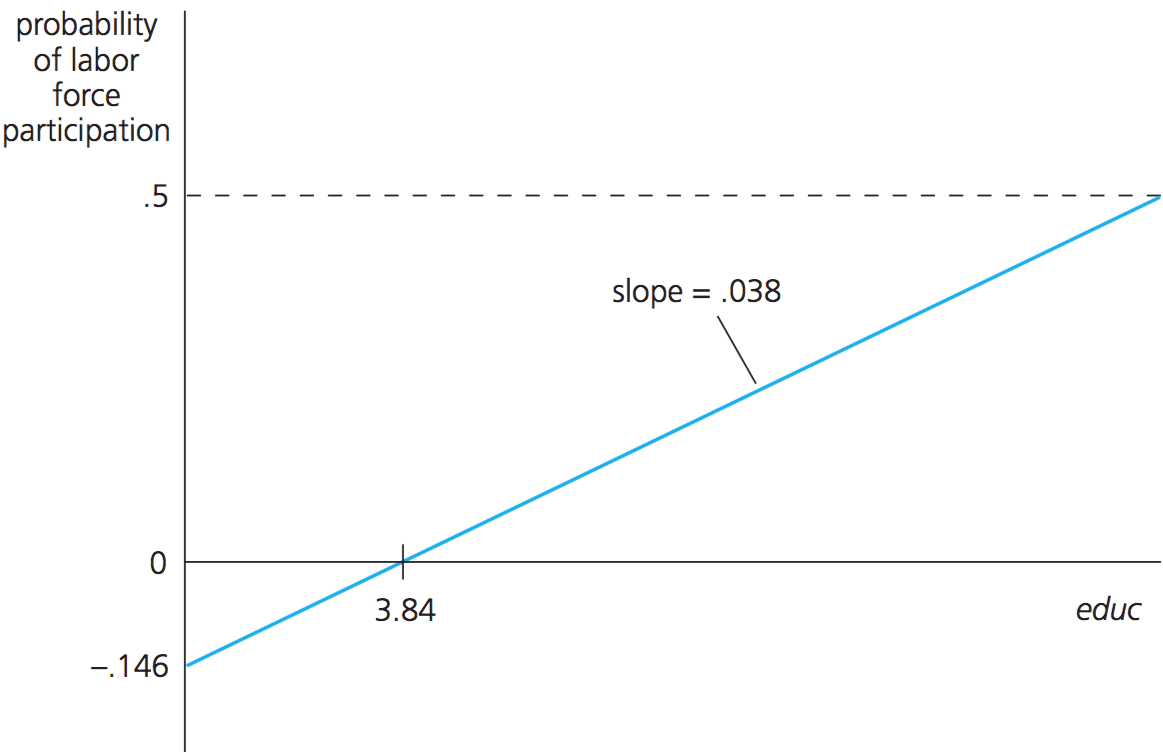
\includegraphics[width=0.75\textwidth,height=\textheight]{"images/Picture1.png"}
\end{frame}

\begin{frame}{Linear Probability Model Drawbacks:}
\protect\hypertarget{linear-probability-model-drawbacks}{}
\begin{enumerate}
[1)]
\item
  The predicted probabilities from our regression aren't bound between 0
  and 1.
\item
  The outcome is implied to be linearly related to the independent
  variables. This is not possible with probabilities. (Ex: going from 0
  to 4 young children reduces the probability by 0.262*4=1.048, 104.8
  percentage points, which is impossible).
\item
  When \(y\) is a binary variable \(Var(y|x)=p(x)[1-p(x)]\). This means
  that there must be heteroskedasticity in the linear probability model.
  Thus you should always use \textbf{heteroskedasticity robust standard
  errors} with linear probability models.
\end{enumerate}
\end{frame}

\hypertarget{logits}{%
\section{Logits}\label{logits}}

\begin{frame}{Logits}
\protect\hypertarget{logits-1}{}
How do we address the drawbacks of linear probability models?

With \textbf{logistic regressions}, which are estimated via maximum
likelihood methods rather than OLS.
\end{frame}

\begin{frame}{Logits}
\protect\hypertarget{logits-2}{}
Logits differ from the linear probability model in the type of function
used for the estimated probability.

In linear probability models, we have

\[
Pr(y=1|x_1, x_2)=\beta_0+\beta_1x_1+\beta_2x_2.
\]

With a logit, we have \[
Pr(y=1|x_1, x_2)=\frac{e^{(\beta_0+\beta_1x_1+\beta_2x_2)}}{1+e^{(\beta_0+\beta_1x_1+\beta_2x_2)}}=\Lambda(\beta_0+\beta_1x_1+\beta_2x_2)
\]

where \(\Lambda\) is commonly used notation to represent the complex
logit function.
\end{frame}

\begin{frame}{Logits}
\protect\hypertarget{logits-3}{}
Why would we ever pick a functional form for the probability that looks
as complicated as \(\Lambda\)?

\begin{itemize}
\item
  Because it is bounded between 0 and 1 (so our predictions make sense),
\item
  it has nice statistical properties (which we will not get into).
\end{itemize}

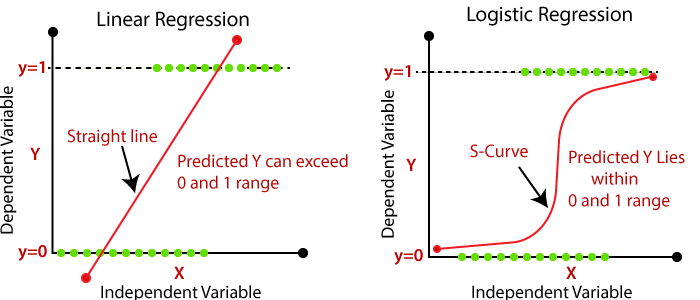
\includegraphics[width=0.75\textwidth,height=\textheight]{"images/lin_v_log.png"}
\end{frame}

\begin{frame}[fragile]{Logits}
\protect\hypertarget{logits-4}{}
In linear probability models, the marginal effect,
\(\frac{\partial Pr(y=1|x)}{\partial x_j}\), of \(x_j\) on \(Pr(y=1|x)\)
is constant.

Logit models are \textbf{non-linear}: the exact marginal effect of
\(x_j\) on \(Pr(y=1|x)\) \textbf{changes depending on the other values
of x}.

We can select where we calculate the marginal effects at:

\begin{itemize}
\item
  In \texttt{R}, the default is to compute the \textbf{average marginal
  effect} which is the average of the marginal effect for each
  observation in the sample.
\item
  we could also specify any values of our independent variables to
  evaluate our marginal effects precisely at those values (Ex: at the
  mean values of the \(x_j\)'s).
\end{itemize}
\end{frame}

\begin{frame}[fragile]{Logits}
\protect\hypertarget{logits-5}{}
Working with Logits:

\begin{itemize}
\item
  \texttt{R} output for a logit will not give you a marginal effect.
  Instead it reports the \textbf{log-odds}.
\item
  To get marginal effects, we need to request the marginal effects and
  specify which marginal effects we are interested.
\end{itemize}
\end{frame}

\begin{frame}[fragile]{Logits}
\protect\hypertarget{logits-6}{}
Looking at labor force participation using the \texttt{mroz} data.

\begin{enumerate}
[1)]
\item
  estimate a logistic regression with the \texttt{glm()} function.
\item
  Running \texttt{summary()} will then get us the log-odds.
\end{enumerate}

\tiny

\begin{Shaded}
\begin{Highlighting}[]
\NormalTok{reglogit1}\OtherTok{\textless{}{-}}\FunctionTok{glm}\NormalTok{(inlf}\SpecialCharTok{\textasciitilde{}}\NormalTok{nwifeinc}\SpecialCharTok{+}\NormalTok{educ}\SpecialCharTok{+}\NormalTok{exper}\SpecialCharTok{+}\NormalTok{exper2}\SpecialCharTok{+}\NormalTok{age}\SpecialCharTok{+}\NormalTok{kidslt6}\SpecialCharTok{+}\NormalTok{kidsge6, mroz, }\AttributeTok{family=}\StringTok{"binomial"}\NormalTok{)}
\FunctionTok{summary}\NormalTok{(reglogit1)}
\end{Highlighting}
\end{Shaded}

\begin{verbatim}
## 
## Call:
## glm(formula = inlf ~ nwifeinc + educ + exper + exper2 + age + 
##     kidslt6 + kidsge6, family = "binomial", data = mroz)
## 
## Deviance Residuals: 
##     Min       1Q   Median       3Q      Max  
## -2.1770  -0.9063   0.4473   0.8561   2.4032  
## 
## Coefficients:
##              Estimate Std. Error z value Pr(>|z|)    
## (Intercept)  0.425452   0.860365   0.495  0.62095    
## nwifeinc    -0.021345   0.008421  -2.535  0.01126 *  
## educ         0.221170   0.043439   5.091 3.55e-07 ***
## exper        0.205870   0.032057   6.422 1.34e-10 ***
## exper2      -0.003154   0.001016  -3.104  0.00191 ** 
## age         -0.088024   0.014573  -6.040 1.54e-09 ***
## kidslt6     -1.443354   0.203583  -7.090 1.34e-12 ***
## kidsge6      0.060112   0.074789   0.804  0.42154    
## ---
## Signif. codes:  0 '***' 0.001 '**' 0.01 '*' 0.05 '.' 0.1 ' ' 1
## 
## (Dispersion parameter for binomial family taken to be 1)
## 
##     Null deviance: 1029.75  on 752  degrees of freedom
## Residual deviance:  803.53  on 745  degrees of freedom
## AIC: 819.53
## 
## Number of Fisher Scoring iterations: 4
\end{verbatim}
\end{frame}

\begin{frame}[fragile]{Logits}
\protect\hypertarget{logits-7}{}
To get the marginal effects:

\begin{enumerate}
[1)]
\setcounter{enumi}{2}
\tightlist
\item
  run the estimated \texttt{glm()} object through the \texttt{margins()}
  function (from the \textbf{margins} package).
\end{enumerate}

\begin{itemize}
\tightlist
\item
  the default returns the \textbf{average marginal effect}
\end{itemize}

\tiny

\begin{Shaded}
\begin{Highlighting}[]
\FunctionTok{library}\NormalTok{(margins)}
\end{Highlighting}
\end{Shaded}

\begin{verbatim}
## Warning: package 'margins' was built under R version 4.1.3
\end{verbatim}

\begin{Shaded}
\begin{Highlighting}[]
\NormalTok{marg\_reglogit1}\OtherTok{\textless{}{-}}\FunctionTok{margins}\NormalTok{(reglogit1)}
\FunctionTok{summary}\NormalTok{(marg\_reglogit1)}
\end{Highlighting}
\end{Shaded}

\begin{verbatim}
##    factor     AME     SE       z      p   lower   upper
##       age -0.0157 0.0024 -6.6027 0.0000 -0.0204 -0.0111
##      educ  0.0395 0.0073  5.4145 0.0000  0.0252  0.0538
##     exper  0.0368 0.0052  7.1386 0.0000  0.0267  0.0469
##    exper2 -0.0006 0.0002 -3.1759 0.0015 -0.0009 -0.0002
##   kidsge6  0.0107 0.0133  0.8051 0.4207 -0.0154  0.0369
##   kidslt6 -0.2578 0.0319 -8.0696 0.0000 -0.3204 -0.1951
##  nwifeinc -0.0038 0.0015 -2.5714 0.0101 -0.0067 -0.0009
\end{verbatim}
\end{frame}

\begin{frame}[fragile]{Logits}
\protect\hypertarget{logits-8}{}
\begin{itemize}
\tightlist
\item
  you can instead compute the marginal effect for a particular type of
  observation:
\end{itemize}

\tiny

\begin{Shaded}
\begin{Highlighting}[]
\NormalTok{DF }\OtherTok{\textless{}{-}} \FunctionTok{data.frame}\NormalTok{(}\AttributeTok{age=}\DecValTok{30}\NormalTok{, }
                 \AttributeTok{nwifeinc=}\DecValTok{50}\NormalTok{,}
                 \AttributeTok{exper=}\DecValTok{5}\NormalTok{,}
                 \AttributeTok{exper2=}\DecValTok{25}\NormalTok{,}
                 \AttributeTok{kidsge6=}\DecValTok{0}\NormalTok{,}
                 \AttributeTok{kidslt6=}\DecValTok{1}\NormalTok{,}
                 \AttributeTok{educ=}\DecValTok{12}\NormalTok{,}
                 \AttributeTok{stringsAsFactors=}\ConstantTok{FALSE}\NormalTok{)}
              
\NormalTok{marg\_specific }\OtherTok{\textless{}{-}} \FunctionTok{margins}\NormalTok{(reglogit1, }\AttributeTok{data =}\NormalTok{ DF)}

\FunctionTok{summary}\NormalTok{(marg\_specific)}
\end{Highlighting}
\end{Shaded}

\begin{verbatim}
##    factor     AME     SE       z      p   lower   upper
##       age -0.0163 0.0049 -3.3268 0.0009 -0.0259 -0.0067
##      educ  0.0410 0.0088  4.6729 0.0000  0.0238  0.0582
##     exper  0.0382 0.0089  4.2893 0.0000  0.0207  0.0556
##    exper2 -0.0006 0.0002 -2.8205 0.0048 -0.0010 -0.0002
##   kidsge6  0.0111 0.0130  0.8554 0.3924 -0.0144  0.0367
##   kidslt6 -0.2675 0.0567 -4.7195 0.0000 -0.3787 -0.1564
##  nwifeinc -0.0040 0.0011 -3.5885 0.0003 -0.0061 -0.0018
\end{verbatim}
\end{frame}

\begin{frame}{Contrasting a logit to a linear probability model (LPM)}
\protect\hypertarget{contrasting-a-logit-to-a-linear-probability-model-lpm}{}
In sports betting, the Las Vegas point spread is the predicted scoring
differential between two opponents as quoted in Las Vegas. We are
interested in the probability that the favored team actually wins.

We can run the following regression: \[
\widehat{favwin}_i=\hat{\beta}_0+\hat{\beta}_1spread_i+\hat{\beta}_2favhome_i+\hat{\beta}_3fav25_i+\hat{\beta}_4und25_i+\hat{u}_i
\]

\begin{itemize}
\item
  \(favwin\) is a dummy variable indicating whether the favored team
  won,
\item
  \(spread\) is the Las Vegas point spread,
\item
  \(favhome\) is a dummy variable indicating whether the favored team is
  playing at home,
\item
  \(fav25\) and \(und25\) indicate whether the favored team and the
  underdog team are in the top 25 teams respectively.
\end{itemize}
\end{frame}

\begin{frame}[fragile]{Logit vs.~linear probability model}
\protect\hypertarget{logit-vs.-linear-probability-model}{}
Using the \texttt{pntsprd} data from the wooldridge package: \tiny

\begin{Shaded}
\begin{Highlighting}[]
\NormalTok{lpm}\OtherTok{\textless{}{-}}\FunctionTok{felm}\NormalTok{(favwin}\SpecialCharTok{\textasciitilde{}}\NormalTok{spread}\SpecialCharTok{+}\NormalTok{favhome}\SpecialCharTok{+}\NormalTok{fav25}\SpecialCharTok{+}\NormalTok{und25, }\AttributeTok{data=}\NormalTok{pntsprd)}
\FunctionTok{summary}\NormalTok{(lpm, }\AttributeTok{robust=}\ConstantTok{TRUE}\NormalTok{)}
\end{Highlighting}
\end{Shaded}

\begin{verbatim}
## 
## Call:
##    felm(formula = favwin ~ spread + favhome + fav25 + und25, data = pntsprd) 
## 
## Residuals:
##     Min      1Q  Median      3Q     Max 
## -0.9972 -0.1105  0.1470  0.2991  0.4869 
## 
## Coefficients:
##              Estimate Robust s.e t value Pr(>|t|)    
## (Intercept)  0.558815   0.040422  13.825   <2e-16 ***
## spread       0.017763   0.002056   8.637   <2e-16 ***
## favhome      0.054353   0.040923   1.328    0.185    
## fav25        0.010982   0.039100   0.281    0.779    
## und25       -0.101104   0.089530  -1.129    0.259    
## ---
## Signif. codes:  0 '***' 0.001 '**' 0.01 '*' 0.05 '.' 0.1 ' ' 1
## 
## Residual standard error: 0.4016 on 548 degrees of freedom
## Multiple R-squared(full model): 0.116   Adjusted R-squared: 0.1095 
## Multiple R-squared(proj model): 0.116   Adjusted R-squared: 0.1095 
## F-statistic(full model, *iid*):17.97 on 4 and 548 DF, p-value: 7.007e-14 
## F-statistic(proj model):  26.2 on 4 and 548 DF, p-value: < 2.2e-16
\end{verbatim}
\end{frame}

\begin{frame}[fragile]{Logit vs.~linear probability model}
\protect\hypertarget{logit-vs.-linear-probability-model-1}{}
\footnotesize

\begin{Shaded}
\begin{Highlighting}[]
\NormalTok{logit}\OtherTok{\textless{}{-}}\FunctionTok{glm}\NormalTok{(favwin}\SpecialCharTok{\textasciitilde{}}\NormalTok{spread}\SpecialCharTok{+}\NormalTok{favhome}\SpecialCharTok{+}\NormalTok{fav25}\SpecialCharTok{+}\NormalTok{und25, }
           \AttributeTok{data=}\NormalTok{pntsprd, }\AttributeTok{family=}\StringTok{"binomial"}\NormalTok{)}
\NormalTok{marg\_logit}\OtherTok{\textless{}{-}}\FunctionTok{margins}\NormalTok{(logit)}
\FunctionTok{summary}\NormalTok{(marg\_logit)}
\end{Highlighting}
\end{Shaded}

\begin{verbatim}
##   factor     AME     SE       z      p   lower  upper
##    fav25  0.0076 0.0434  0.1748 0.8612 -0.0774 0.0926
##  favhome  0.0425 0.0362  1.1740 0.2404 -0.0284 0.1134
##   spread  0.0243 0.0033  7.3360 0.0000  0.0178 0.0308
##    und25 -0.0579 0.0650 -0.8912 0.3728 -0.1852 0.0694
\end{verbatim}
\end{frame}

\begin{frame}{Logit vs.~linear probability model}
\protect\hypertarget{logit-vs.-linear-probability-model-2}{}
All else constant, a 1 point increase in the Vegas point spread is
estimated to increase the predicted probability of winning:

\begin{itemize}
\item
  by 1.78 percentage points using the linear probability model
\item
  by 2.43 percentage points on average using the logit model.
\end{itemize}

It is generally the case that results using these two different methods
will often be quite similar.
\end{frame}

\begin{frame}[fragile]{Logit vs.~linear probability model}
\protect\hypertarget{logit-vs.-linear-probability-model-3}{}
To see the difference, we plot the predicted probabilities

\small

\begin{Shaded}
\begin{Highlighting}[]
\CommentTok{\#generating the fitted values for both models}
\NormalTok{df}\OtherTok{\textless{}{-}} \FunctionTok{mutate}\NormalTok{(pntsprd, }\AttributeTok{lpm\_prob=}\NormalTok{lpm}\SpecialCharTok{$}\NormalTok{fitted.values,}
            \AttributeTok{logit\_prob=}\NormalTok{logit}\SpecialCharTok{$}\NormalTok{fitted.values)}

\NormalTok{plot}\OtherTok{\textless{}{-}}\NormalTok{df}\SpecialCharTok{\%\textgreater{}\%}
  \FunctionTok{ggplot}\NormalTok{(}\FunctionTok{aes}\NormalTok{(}\AttributeTok{x=}\NormalTok{spread))}\SpecialCharTok{+}
  \FunctionTok{geom\_point}\NormalTok{(}\FunctionTok{aes}\NormalTok{(}\AttributeTok{y=}\NormalTok{lpm\_prob, }\AttributeTok{colour=}\StringTok{"LPM"}\NormalTok{), }\AttributeTok{alpha=}\FloatTok{0.6}\NormalTok{)}\SpecialCharTok{+}
  \FunctionTok{geom\_point}\NormalTok{(}\FunctionTok{aes}\NormalTok{(}\AttributeTok{y=}\NormalTok{logit\_prob, }\AttributeTok{colour=}\StringTok{"Logit"}\NormalTok{), }\AttributeTok{alpha=}\FloatTok{0.6}\NormalTok{)}\SpecialCharTok{+}
  \FunctionTok{geom\_hline}\NormalTok{(}\AttributeTok{yintercept =} \DecValTok{1}\NormalTok{, }\AttributeTok{alpha=}\FloatTok{0.7}\NormalTok{)}\SpecialCharTok{+}
  \FunctionTok{geom\_hline}\NormalTok{(}\AttributeTok{yintercept =} \DecValTok{0}\NormalTok{,}\AttributeTok{alpha=}\FloatTok{0.7}\NormalTok{)}\SpecialCharTok{+}
  \FunctionTok{scale\_colour\_manual}\NormalTok{(}\StringTok{"Model"}\NormalTok{,}
                      \AttributeTok{breaks=}\FunctionTok{c}\NormalTok{(}\StringTok{"LPM"}\NormalTok{, }\StringTok{"Logit"}\NormalTok{),}
                      \AttributeTok{values=}\FunctionTok{c}\NormalTok{(}\StringTok{"blue"}\NormalTok{, }\StringTok{"forestgreen"}\NormalTok{))}\SpecialCharTok{+}
  \FunctionTok{lims}\NormalTok{(}\AttributeTok{y=}\FunctionTok{c}\NormalTok{(}\DecValTok{0}\NormalTok{,}\FloatTok{1.4}\NormalTok{))}\SpecialCharTok{+}
  \FunctionTok{labs}\NormalTok{(}\AttributeTok{title=}\StringTok{"Predicted Win Probabilities, LPM"}\NormalTok{,}
       \AttributeTok{x=}\StringTok{"Spread"}\NormalTok{,}
       \AttributeTok{y=}\StringTok{"Probability"}\NormalTok{)}
\end{Highlighting}
\end{Shaded}
\end{frame}

\begin{frame}[fragile]{Logit vs.~linear probability model}
\protect\hypertarget{logit-vs.-linear-probability-model-4}{}
\begin{Shaded}
\begin{Highlighting}[]
\NormalTok{plot}
\end{Highlighting}
\end{Shaded}

\includegraphics{Slides_Misc_files/figure-beamer/logitvlpm4-1.pdf}
\end{frame}

\hypertarget{non-standard-standard-errors}{%
\section{Non-standard standard
errors}\label{non-standard-standard-errors}}

\begin{frame}{Non-standard standard errors}
\protect\hypertarget{non-standard-standard-errors-1}{}
A standard error estimates the uncertainty around an estimated
parameter.

Formally we have \[
se=\sqrt{\widehat{Var(\hat{\beta})}}. 
\]

Just like calculating point estimates, it is incredibly important to get
your standard errors right.

You have to know what you don't know!

\begin{itemize}
\item
  Robust standard errors
\item
  Clustered standard errors
\item
  Newey-West Standard Errors
\item
  Conley Standard Errors
\end{itemize}
\end{frame}

\hypertarget{robust-standard-errors}{%
\section{Robust Standard errors}\label{robust-standard-errors}}

\begin{frame}[fragile]{Robust standard errors}
\protect\hypertarget{robust-standard-errors-1}{}
Using the diamonds data set from \texttt{ggplot2}:

\tiny

\begin{Shaded}
\begin{Highlighting}[]
\NormalTok{knitr}\SpecialCharTok{::}\FunctionTok{kable}\NormalTok{(}\FunctionTok{head}\NormalTok{(diamonds))}
\end{Highlighting}
\end{Shaded}

\begin{longtable}[]{@{}
  >{\raggedleft\arraybackslash}p{(\columnwidth - 18\tabcolsep) * \real{0.0952}}
  >{\raggedright\arraybackslash}p{(\columnwidth - 18\tabcolsep) * \real{0.1587}}
  >{\raggedright\arraybackslash}p{(\columnwidth - 18\tabcolsep) * \real{0.0952}}
  >{\raggedright\arraybackslash}p{(\columnwidth - 18\tabcolsep) * \real{0.1270}}
  >{\raggedleft\arraybackslash}p{(\columnwidth - 18\tabcolsep) * \real{0.0952}}
  >{\raggedleft\arraybackslash}p{(\columnwidth - 18\tabcolsep) * \real{0.0952}}
  >{\raggedleft\arraybackslash}p{(\columnwidth - 18\tabcolsep) * \real{0.0952}}
  >{\raggedleft\arraybackslash}p{(\columnwidth - 18\tabcolsep) * \real{0.0794}}
  >{\raggedleft\arraybackslash}p{(\columnwidth - 18\tabcolsep) * \real{0.0794}}
  >{\raggedleft\arraybackslash}p{(\columnwidth - 18\tabcolsep) * \real{0.0794}}@{}}
\toprule()
\begin{minipage}[b]{\linewidth}\raggedleft
carat
\end{minipage} & \begin{minipage}[b]{\linewidth}\raggedright
cut
\end{minipage} & \begin{minipage}[b]{\linewidth}\raggedright
color
\end{minipage} & \begin{minipage}[b]{\linewidth}\raggedright
clarity
\end{minipage} & \begin{minipage}[b]{\linewidth}\raggedleft
depth
\end{minipage} & \begin{minipage}[b]{\linewidth}\raggedleft
table
\end{minipage} & \begin{minipage}[b]{\linewidth}\raggedleft
price
\end{minipage} & \begin{minipage}[b]{\linewidth}\raggedleft
x
\end{minipage} & \begin{minipage}[b]{\linewidth}\raggedleft
y
\end{minipage} & \begin{minipage}[b]{\linewidth}\raggedleft
z
\end{minipage} \\
\midrule()
\endhead
0.23 & Ideal & E & SI2 & 61.5 & 55 & 326 & 3.95 & 3.98 & 2.43 \\
0.21 & Premium & E & SI1 & 59.8 & 61 & 326 & 3.89 & 3.84 & 2.31 \\
0.23 & Good & E & VS1 & 56.9 & 65 & 327 & 4.05 & 4.07 & 2.31 \\
0.29 & Premium & I & VS2 & 62.4 & 58 & 334 & 4.20 & 4.23 & 2.63 \\
0.31 & Good & J & SI2 & 63.3 & 58 & 335 & 4.34 & 4.35 & 2.75 \\
0.24 & Very Good & J & VVS2 & 62.8 & 57 & 336 & 3.94 & 3.96 & 2.48 \\
\bottomrule()
\end{longtable}
\end{frame}

\begin{frame}[fragile]{Robust standard errors}
\protect\hypertarget{robust-standard-errors-2}{}
Regress price on carats and depth.

\tiny

\begin{Shaded}
\begin{Highlighting}[]
\NormalTok{reg1}\OtherTok{\textless{}{-}}\FunctionTok{felm}\NormalTok{(price}\SpecialCharTok{\textasciitilde{}}\NormalTok{carat}\SpecialCharTok{+}\NormalTok{depth, diamonds)}

\FunctionTok{summary}\NormalTok{(reg1)}
\end{Highlighting}
\end{Shaded}

\begin{verbatim}
## 
## Call:
##    felm(formula = price ~ carat + depth, data = diamonds) 
## 
## Residuals:
##      Min       1Q   Median       3Q      Max 
## -18238.9   -801.6    -19.6    546.3  12683.7 
## 
## Coefficients:
##             Estimate Std. Error t value Pr(>|t|)    
## (Intercept) 4045.333    286.205   14.13   <2e-16 ***
## carat       7765.141     14.009  554.28   <2e-16 ***
## depth       -102.165      4.635  -22.04   <2e-16 ***
## ---
## Signif. codes:  0 '***' 0.001 '**' 0.01 '*' 0.05 '.' 0.1 ' ' 1
## 
## Residual standard error: 1542 on 53937 degrees of freedom
## Multiple R-squared(full model): 0.8507   Adjusted R-squared: 0.8507 
## Multiple R-squared(proj model): 0.8507   Adjusted R-squared: 0.8507 
## F-statistic(full model):1.536e+05 on 2 and 53937 DF, p-value: < 2.2e-16 
## F-statistic(proj model): 1.536e+05 on 2 and 53937 DF, p-value: < 2.2e-16
\end{verbatim}
\end{frame}

\begin{frame}[fragile]{Robust standard errors}
\protect\hypertarget{robust-standard-errors-3}{}
Cool.

Plot the data to check OLS assumptions:

\tiny

\begin{Shaded}
\begin{Highlighting}[]
\NormalTok{myPlot }\OtherTok{\textless{}{-}} \FunctionTok{ggplot}\NormalTok{(}\AttributeTok{data =}\NormalTok{ diamonds, }\FunctionTok{aes}\NormalTok{(}\AttributeTok{y =}\NormalTok{ price, }\AttributeTok{x =}\NormalTok{ carat)) }\SpecialCharTok{+}
\FunctionTok{geom\_point}\NormalTok{(}\AttributeTok{color =} \StringTok{"gray50"}\NormalTok{, }\AttributeTok{shape =} \DecValTok{21}\NormalTok{) }
\end{Highlighting}
\end{Shaded}
\end{frame}

\begin{frame}{Robust standard errors}
\protect\hypertarget{robust-standard-errors-4}{}
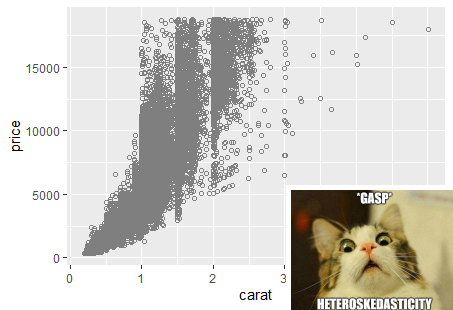
\includegraphics[width=6.29in]{img_with_inset}
\end{frame}

\begin{frame}{Robust standard errors}
\protect\hypertarget{robust-standard-errors-5}{}
You should have the econometric heebie jeebies.

Homoskedastic assumption needed for OLS is not valid!

\begin{itemize}
\item
  The higher the carat, the greater the variance in price.
\item
  \(\Rightarrow\) OLS standard errors are likely to be wrong.
\end{itemize}

Thankfully all is not lost!
\end{frame}

\begin{frame}{Robust standard errors}
\protect\hypertarget{robust-standard-errors-6}{}
Lets relax the homoskedasticity assumption and allow for the variance to
depend on the value of \(x_i\).

We know that \[
Var(\hat{\beta_1})=\frac{\sigma^2}{\sum_{i=1}^n(x_i-\bar{x})^2}=\frac{\sum_{i=1}^n(x_i-\bar{x})^2\sigma^2}{(\sum_{i=1}^n(x_i-\bar{x})^2)^2}
\]

With heteroskedasticity \(\sigma^2\) is no longer constant and becomes a
function of the particular value of \(x_i\) an observation has, so

\[
Var(u_i|x_i)=\sigma^2_i
\]

Where are we going to find all these \(\sigma_i^2\) for each individual
observation?
\end{frame}

\begin{frame}{Eicker, Huber and White to the rescue!}
\protect\hypertarget{eicker-huber-and-white-to-the-rescue}{}
Econometricians Eicker, Huber and White figured out a way to do this by
basically using the square of the estimated residual of each
observation, \(\hat{u}_i^2\), as a stand-in for \(\sigma^2_i\).

With this trick, a valid estimator for \(Var(\hat{beta_1})\), with
heteroskedasticity of \textbf{any} form (including homoskedasticity), is

\[
Var(\hat{\beta_1})=\frac{\sum_{i=1}^n(x_i-\bar{x})^2\hat{u}_i^2}{(\sum_{i=1}^n(x_i-\bar{x})^2)^2}
\]

We commonly call the resulting standard errors ``robust'', or
``heteroskedasticity-robust''.
\end{frame}

\begin{frame}[fragile]{Robust standard errors}
\protect\hypertarget{robust-standard-errors-7}{}
How can we find these in R?

\tiny

\begin{Shaded}
\begin{Highlighting}[]
\NormalTok{reg1}\OtherTok{\textless{}{-}}\FunctionTok{felm}\NormalTok{(price}\SpecialCharTok{\textasciitilde{}}\NormalTok{carat}\SpecialCharTok{+}\NormalTok{depth, diamonds)}

\FunctionTok{summary}\NormalTok{(reg1, }\AttributeTok{robust=}\ConstantTok{TRUE}\NormalTok{)}
\end{Highlighting}
\end{Shaded}

\begin{verbatim}
## 
## Call:
##    felm(formula = price ~ carat + depth, data = diamonds) 
## 
## Residuals:
##      Min       1Q   Median       3Q      Max 
## -18238.9   -801.6    -19.6    546.3  12683.7 
## 
## Coefficients:
##             Estimate Robust s.e t value Pr(>|t|)    
## (Intercept) 4045.333    369.176   10.96   <2e-16 ***
## carat       7765.141     25.105  309.31   <2e-16 ***
## depth       -102.165      5.946  -17.18   <2e-16 ***
## ---
## Signif. codes:  0 '***' 0.001 '**' 0.01 '*' 0.05 '.' 0.1 ' ' 1
## 
## Residual standard error: 1542 on 53937 degrees of freedom
## Multiple R-squared(full model): 0.8507   Adjusted R-squared: 0.8507 
## Multiple R-squared(proj model): 0.8507   Adjusted R-squared: 0.8507 
## F-statistic(full model, *iid*):1.536e+05 on 2 and 53937 DF, p-value: < 2.2e-16 
## F-statistic(proj model): 4.878e+04 on 2 and 53937 DF, p-value: < 2.2e-16
\end{verbatim}
\end{frame}

\begin{frame}[fragile]{Robust standard errors}
\protect\hypertarget{robust-standard-errors-8}{}
Or if you want to put them in a stargazer table: \tiny 

\begin{Shaded}
\begin{Highlighting}[]
\FunctionTok{stargazer}\NormalTok{(reg1, }\AttributeTok{type =} \StringTok{"latex"}\NormalTok{ , }\AttributeTok{se =}  \FunctionTok{list}\NormalTok{(reg1}\SpecialCharTok{$}\NormalTok{rse), }\AttributeTok{header=}\ConstantTok{FALSE}\NormalTok{)}
\end{Highlighting}
\end{Shaded}

\begin{table}[!htbp] \centering 
  \caption{} 
  \label{} 
\begin{tabular}{@{\extracolsep{5pt}}lc} 
\\[-1.8ex]\hline 
\hline \\[-1.8ex] 
 & \multicolumn{1}{c}{\textit{Dependent variable:}} \\ 
\cline{2-2} 
\\[-1.8ex] & price \\ 
\hline \\[-1.8ex] 
 carat & 7,765.141$^{***}$ \\ 
  & (25.105) \\ 
  & \\ 
 depth & $-$102.165$^{***}$ \\ 
  & (5.946) \\ 
  & \\ 
 Constant & 4,045.333$^{***}$ \\ 
  & (369.176) \\ 
  & \\ 
\hline \\[-1.8ex] 
Observations & 53,940 \\ 
R$^{2}$ & 0.851 \\ 
Adjusted R$^{2}$ & 0.851 \\ 
Residual Std. Error & 1,541.649 (df = 53937) \\ 
\hline 
\hline \\[-1.8ex] 
\textit{Note:}  & \multicolumn{1}{r}{$^{*}$p$<$0.1; $^{**}$p$<$0.05; $^{***}$p$<$0.01} \\ 
\end{tabular} 
\end{table} 
\normalsize

Note: robust standard errors are larger than regular standard errors,
and thus more conservative (which is the right thing to be\ldots{} you
want to know what you don't know).
\end{frame}

\hypertarget{clustered-standard-errors}{%
\section{Clustered standard errors}\label{clustered-standard-errors}}

\begin{frame}{Econometricians Haiku}
\protect\hypertarget{econometricians-haiku}{}
\textbf{\emph{T-stats looks too good}}

\textbf{\emph{Try cluster standard errors}}

\textbf{\emph{significance gone.}}

\bigskip

\small

from Angrist and Pischke 2008
\end{frame}

\begin{frame}{Clustered standard errors}
\protect\hypertarget{clustered-standard-errors-1}{}
Suppose that every observation belongs to (only) one of G groups.

The assumption we make when we cluster:

\begin{itemize}
\item
  there is no correlation across groups
\item
  we allow for arbitrary within-group correlation.
\end{itemize}
\end{frame}

\begin{frame}{Clustered standard errors}
\protect\hypertarget{clustered-standard-errors-2}{}
Example: consider individuals within a village.

It may be reasonable to think that individuals' error terms are:

\begin{itemize}
\item
  correlated within a village
\item
  aren't correlated across villages
\end{itemize}
\end{frame}

\begin{frame}{Clustered standard errors}
\protect\hypertarget{clustered-standard-errors-3}{}
I will spare you the matrix math needed to dive deeper into this.

Suffice to say that ``cluster-robust'' estimates allow for a more
complicated set of correlations to exist within observations within a
cluster.

One thing to be aware of though is that you will need to have a fairly
large number of clusters (40+) for the estimate to be credible.
\end{frame}

\begin{frame}[fragile]{Clustered standard errors}
\protect\hypertarget{clustered-standard-errors-4}{}
Clustering in R:

I use the \texttt{NOxEmissions} dataset from the \texttt{robustbase}
package.

\begin{itemize}
\item
  hourly \(NO_x\) readings, including \(NO_x\) concentration, auto
  emissions and windspeed.
\item
  use the observation date as our cluster variable.
\end{itemize}

This allows for arbitrary dependence between observations in the same
day, and zero correlation across days.

Is this reasonable? \ldots{} Maybe. But we'll go with it for now:
\end{frame}

\begin{frame}[fragile]{Clustered standard errors}
\protect\hypertarget{clustered-standard-errors-5}{}
\tiny

\begin{Shaded}
\begin{Highlighting}[]
\NormalTok{nox }\OtherTok{\textless{}{-}} \FunctionTok{as.data.frame}\NormalTok{(NOxEmissions) }\SpecialCharTok{\%\textgreater{}\%}\FunctionTok{mutate}\NormalTok{(}\AttributeTok{ones =} \DecValTok{1}\NormalTok{)}
\NormalTok{noClusters }\OtherTok{\textless{}{-}} \FunctionTok{felm}\NormalTok{(}\AttributeTok{data =}\NormalTok{ nox, LNOx }\SpecialCharTok{\textasciitilde{}}\NormalTok{ sqrtWS )}
\NormalTok{Clusters }\OtherTok{\textless{}{-}} \FunctionTok{felm}\NormalTok{(}\AttributeTok{data =}\NormalTok{ nox, LNOx }\SpecialCharTok{\textasciitilde{}}\NormalTok{ sqrtWS }\SpecialCharTok{|}\DecValTok{0}\SpecialCharTok{|}\DecValTok{0}\SpecialCharTok{|}\NormalTok{ julday)}
\FunctionTok{stargazer}\NormalTok{(noClusters,Clusters, }\AttributeTok{type =} \StringTok{"latex"}\NormalTok{ , }\AttributeTok{header=}\ConstantTok{FALSE}\NormalTok{, }\AttributeTok{omit.stat =} \StringTok{"all"}\NormalTok{)}
\end{Highlighting}
\end{Shaded}

\begin{table}[!htbp] \centering 
  \caption{} 
  \label{} 
\begin{tabular}{@{\extracolsep{5pt}}lcc} 
\\[-1.8ex]\hline 
\hline \\[-1.8ex] 
 & \multicolumn{2}{c}{\textit{Dependent variable:}} \\ 
\cline{2-3} 
\\[-1.8ex] & \multicolumn{2}{c}{LNOx} \\ 
\\[-1.8ex] & (1) & (2)\\ 
\hline \\[-1.8ex] 
 sqrtWS & $-$0.864$^{***}$ & $-$0.864$^{***}$ \\ 
  & (0.020) & (0.048) \\ 
  & & \\ 
 Constant & 5.559$^{***}$ & 5.559$^{***}$ \\ 
  & (0.029) & (0.065) \\ 
  & & \\ 
\hline \\[-1.8ex] 
\hline 
\hline \\[-1.8ex] 
\textit{Note:}  & \multicolumn{2}{r}{$^{*}$p$<$0.1; $^{**}$p$<$0.05; $^{***}$p$<$0.01} \\ 
\end{tabular} 
\end{table}

\normalsize

Here, the regular standard errors are smaller than the clustered
standard errors.

This need not necessarily be the case and depends on the correlation
between observations within a cluster.
\end{frame}

\begin{frame}{Newey West Standard Errors}
\protect\hypertarget{newey-west-standard-errors}{}
For time series data.
\end{frame}

\begin{frame}{Conley Standard Errors}
\protect\hypertarget{conley-standard-errors}{}
For spatial data.
\end{frame}

\hypertarget{confidence-intervals-for-predictions}{%
\section{Confidence intervals for
predictions}\label{confidence-intervals-for-predictions}}

\begin{frame}{Confidence intervals for predictions}
\protect\hypertarget{confidence-intervals-for-predictions-1}{}
You know how to ``predict'' a value of the dependent variable, \(y\),
given certain values of the independent variables.

This prediction is just a guess, with uncertainty.

We can construct a confidence interval to give a range of possible
values for this prediction.

There are two kinds of predictions we can make:

\begin{itemize}
\item
  A confidence interval for the \textbf{average} \(y\) given \(x_1\),
  \(x_2\)\ldots{} \(x_k\).
\item
  A confidence interval for a \textbf{particular} \(y\) given \(x_1\),
  \(x_2\)\ldots{} \(x_k\).
\end{itemize}
\end{frame}

\begin{frame}{Confidence intervals for predictions}
\protect\hypertarget{confidence-intervals-for-predictions-2}{}
Using Wooldridge's birth weight data:

\[
bweight=\beta_0+\beta_1lfaminc+\beta_2 meduc+\beta_3 parity+u
\]

\begin{itemize}
\item
  bwght is birth weight in ounces,
\item
  lfaminc is the log of family income in \$1000s,
\item
  meduc is the education of the mother in years,
\item
  parity is the birth order of the child.
\end{itemize}
\end{frame}

\begin{frame}[fragile]{Confidence intervals for predictions}
\protect\hypertarget{confidence-intervals-for-predictions-3}{}
Estimating this equation in R, we get the following results:

\tiny

\begin{Shaded}
\begin{Highlighting}[]
\CommentTok{\#using the bwght data from the wooldridge package}
\NormalTok{reg1}\OtherTok{\textless{}{-}}\FunctionTok{lm}\NormalTok{(bwght}\SpecialCharTok{\textasciitilde{}}\NormalTok{lfaminc}\SpecialCharTok{+}\NormalTok{motheduc}\SpecialCharTok{+}\NormalTok{parity, bwght)}

\FunctionTok{summary}\NormalTok{(reg1)}
\end{Highlighting}
\end{Shaded}

\begin{verbatim}
## 
## Call:
## lm(formula = bwght ~ lfaminc + motheduc + parity, data = bwght)
## 
## Residuals:
##     Min      1Q  Median      3Q     Max 
## -94.533 -11.888   0.779  13.136 151.477 
## 
## Coefficients:
##             Estimate Std. Error t value Pr(>|t|)    
## (Intercept) 105.5652     3.3666  31.356  < 2e-16 ***
## lfaminc       2.1313     0.6506   3.276  0.00108 ** 
## motheduc      0.3172     0.2520   1.259  0.20829    
## parity        1.5261     0.6119   2.494  0.01275 *  
## ---
## Signif. codes:  0 '***' 0.001 '**' 0.01 '*' 0.05 '.' 0.1 ' ' 1
## 
## Residual standard error: 20.21 on 1383 degrees of freedom
##   (1 observation deleted due to missingness)
## Multiple R-squared:  0.01633,    Adjusted R-squared:  0.0142 
## F-statistic: 7.654 on 3 and 1383 DF,  p-value: 4.482e-05
\end{verbatim}
\end{frame}

\begin{frame}{Confidence intervals for predictions: for a specific
average}
\protect\hypertarget{confidence-intervals-for-predictions-for-a-specific-average}{}
Our model gives us the expected value: \small \[
E[bweight|faminc, meduc, parity]=\beta_0+\beta_1log(faminc)+\beta_2meduc+\beta_3parity
\] \normalsize and our regression gives us an estimate of this:
\footnotesize \[
\hat{E}[bweight|faminc, meduc,parity]=\hat{y}=\hat{\beta_0}+\hat{\beta_1}log(faminc)+\hat{\beta_2}meduc+\hat{\beta_3}parity
\] \normalsize \(\hat{y}\) is the expected value of y given the
particular values for the explanatory variables.
\end{frame}

\begin{frame}{Confidence intervals for predictions: for a specific
average}
\protect\hypertarget{confidence-intervals-for-predictions-for-a-specific-average-1}{}
Say we are interested in a confidence interval for the \textbf{average
birthweight} for babies with:

\begin{itemize}
\item
  a family income of \$14,500 (ln(14.5)=2.674),
\item
  mothers with 12 years of education,
\item
  2 older siblings (parity=3). \tiny \[
  \begin{aligned}
  \hat{E}[bweight|faminc=14.5, meduc=12, parity=3]&=105.66+2.13ln(faminc)+0.317meduc+1.53parity\\
  \hat{y}_{faminc=14.5, meduc=12, parity=3} &= 105.66+2.13 (2.674)+0.317(12)+1.53(3)\\
  &= 119.75 ounces
  \end{aligned}
  \] \normalsize How do we find a standard error for \(\hat{y}\) at
  these particular values of the explanatory variables?
\end{itemize}
\end{frame}

\begin{frame}{Confidence intervals for predictions: for a specific
average}
\protect\hypertarget{confidence-intervals-for-predictions-for-a-specific-average-2}{}
This standard error is complicated because \(\widehat{bweight}\) is a
function of our \(\hat{\beta}\)'s which are all random variables.

To avoid this computation, we want to transform our data.
\end{frame}

\begin{frame}{Confidence intervals for predictions: for a specific
average}
\protect\hypertarget{confidence-intervals-for-predictions-for-a-specific-average-3}{}
Recall that we have the following regression in mind \[
bweight=\beta_0+\beta_1lfaminc+\beta_2 meduc+\beta_3 parity+u
\] Then \[
\hat{\beta_0}=\hat{E}(bweight|lfaminc=0, meduc=0, parity=0)
\]
\end{frame}

\begin{frame}[fragile]{Confidence intervals for predictions: for a
specific average}
\protect\hypertarget{confidence-intervals-for-predictions-for-a-specific-average-4}{}
If we modify the regression by subtracting our particular values from
the independent variables, we get \[
bweight=\beta_0+\beta_1(lfaminc-2.674)+\beta_2(meduc-12)+\beta_3(parity-3)+u
\] Then \[
\hat{\beta_0}=\hat{E}(bweight|lfaminc=2.674, meduc=12, parity=3).
\]

The new intercept is the predicted birthweight for babies with the
particular values we are interested in.

If we run this regression in \texttt{R}, we can then grab the standard
errors for the intercept.
\end{frame}

\begin{frame}{Confidence intervals for predictions: for a specific
average}
\protect\hypertarget{confidence-intervals-for-predictions-for-a-specific-average-5}{}
So step by step we need to:

\begin{enumerate}
[1)]
\item
  Generate new variables: \(\tilde{x}_j=x_j-\alpha_j\)
\item
  Run the regression:
  \(y=\tilde{\beta_0}+\tilde{\beta_1}\tilde{x_1}+...+\tilde{\beta_k}\tilde{x_k}+\tilde{u}\)
\item
  Then \(\hat{E}[y|x_1=\alpha_1,...,x_k=\alpha_k]=\tilde{\beta_0}\)
\item
  Plug these values into the formula for confidence intervals and
  interpret.
\end{enumerate}
\end{frame}

\begin{frame}[fragile]{Confidence intervals for predictions: for a
specific average}
\protect\hypertarget{confidence-intervals-for-predictions-for-a-specific-average-6}{}
\tiny

\begin{Shaded}
\begin{Highlighting}[]
\CommentTok{\#Step 1: generate new variables}
\NormalTok{bwght}\SpecialCharTok{$}\NormalTok{lfaminc\_0}\OtherTok{\textless{}{-}}\NormalTok{bwght}\SpecialCharTok{$}\NormalTok{lfaminc}\FloatTok{{-}2.674}
\NormalTok{bwght}\SpecialCharTok{$}\NormalTok{motheduc\_0}\OtherTok{\textless{}{-}}\NormalTok{bwght}\SpecialCharTok{$}\NormalTok{motheduc}\DecValTok{{-}12}
\NormalTok{bwght}\SpecialCharTok{$}\NormalTok{parity\_0}\OtherTok{\textless{}{-}}\NormalTok{bwght}\SpecialCharTok{$}\NormalTok{parity}\DecValTok{{-}3}

\CommentTok{\#step 2: run the new regression}
\NormalTok{reg2}\OtherTok{\textless{}{-}}\FunctionTok{lm}\NormalTok{(bwght}\SpecialCharTok{\textasciitilde{}}\NormalTok{lfaminc\_0}\SpecialCharTok{+}\NormalTok{motheduc\_0}\SpecialCharTok{+}\NormalTok{parity\_0,bwght)}

\FunctionTok{summary}\NormalTok{(reg2)}
\end{Highlighting}
\end{Shaded}

\begin{verbatim}
## 
## Call:
## lm(formula = bwght ~ lfaminc_0 + motheduc_0 + parity_0, data = bwght)
## 
## Residuals:
##     Min      1Q  Median      3Q     Max 
## -94.533 -11.888   0.779  13.136 151.477 
## 
## Coefficients:
##             Estimate Std. Error t value Pr(>|t|)    
## (Intercept) 119.6491     1.0066 118.864  < 2e-16 ***
## lfaminc_0     2.1313     0.6506   3.276  0.00108 ** 
## motheduc_0    0.3172     0.2520   1.259  0.20829    
## parity_0      1.5261     0.6119   2.494  0.01275 *  
## ---
## Signif. codes:  0 '***' 0.001 '**' 0.01 '*' 0.05 '.' 0.1 ' ' 1
## 
## Residual standard error: 20.21 on 1383 degrees of freedom
##   (1 observation deleted due to missingness)
## Multiple R-squared:  0.01633,    Adjusted R-squared:  0.0142 
## F-statistic: 7.654 on 3 and 1383 DF,  p-value: 4.482e-05
\end{verbatim}
\end{frame}

\begin{frame}{Confidence intervals for predictions: for a specific
average}
\protect\hypertarget{confidence-intervals-for-predictions-for-a-specific-average-7}{}
The 95\% confidence interval for the average birthweight for babies
given a family income of \$14,500, a mother with 12 years of education
and with 2 older siblings is:

\[
[119.64-1.96(1.007), 119.64+1.96(1.007)]=[117.6653,121.6158]
\]
\end{frame}

\begin{frame}{Confidence Interval for prediction: a specific unit}
\protect\hypertarget{confidence-interval-for-prediction-a-specific-unit}{}
A confidence interval for a particular average is not the same as a
confidence interval for a particular individual.

For individual observations, we must account for the variance in the
unobserved error, \(u_i\), which measures our ignorance of the
unobserved factors that affect \(y_i\).
\end{frame}

\begin{frame}{Confidence Interval for prediction: a specific unit}
\protect\hypertarget{confidence-interval-for-prediction-a-specific-unit-1}{}
We want a confidence interval for \(bweight_{i=1}\), the birthweight of
baby \(i=1\), with \[
bweight_{i=1}=\beta_0+\beta_1lfaminc_{i=1}+\beta_2meduc_{i=1}+\beta_3parity_{i=1}+u_{i=1}
\] Our best prediction of \(bweight_{i=1}\) is
\(\widehat{bwieght}_{i=1}\) where \[
\widehat{bweight}_{i=1}=\hat{\beta}_0+\hat{\beta}_1lfaminc_{i=1}+\hat{\beta}_2meduc_{i=1}+\hat{\beta}_3parity_{i=1}
\]
\end{frame}

\begin{frame}{Confidence Interval for prediction: a specific unit}
\protect\hypertarget{confidence-interval-for-prediction-a-specific-unit-2}{}
There is some error, \(\hat{u}_{i=1}\), associated with using
\(\widehat{bweight}_{i=1}\) to predict \(bweight_{i=1}\) where

\[
\begin{aligned}
\hat{u}_{i=1}&=bweight_{i=1}-\widehat{bweight}_{i=1}\\
&=(\beta_0+\beta_1lfaminc_{i=1}+\beta_2meduc_{i=1}+\beta_3parity_{i=1}+u_{i=1})\\
&-(\hat{\beta}_0+\hat{\beta}_1lfaminc_{i=1}+\hat{\beta}_2meduc_{i=1}+\hat{\beta}_3parity_{i=1})
\end{aligned}
\]

Finding the expected value, we get: \footnotesize \[
\begin{aligned}
E[\hat{u}_{i=1}]&=E[bweight_{i=1}-\widehat{bweight}_{i=1}]\\
&=(\beta_0+\beta_1lfaminc_{i=1}+\beta_2meduc_{i=1}+\beta_3parity_{i=1}+E[u_{i=1}])\\
&-(E[\hat{\beta}_0]+E[\hat{\beta}_1]lfaminc_{i=1}+E[\hat{\beta}_2]meduc_{i=1}+E[\hat{\beta}_3]parity_{i=1})\\
&=0
\end{aligned}
\]
\end{frame}

\begin{frame}{Confidence Interval for prediction: a specific unit}
\protect\hypertarget{confidence-interval-for-prediction-a-specific-unit-3}{}
Finding the variance we get \footnotesize \[
\begin{aligned}
Var(\hat{u}_{i=1})&=Var(bweight_{i=1}-\widehat{bweight}_{i=1})\\
&=Var(\beta_0+\beta_1lfaminc_{i=1}+\beta_2meduc_{i=1}+\beta_3parity_{i=1}+u_{i=1}-\widehat{bweight}_{i=1})\\
&=Var(\widehat{bweight}_{i=1})+Var(u_{i=1})\\
&=Var(\widehat{bweight}_{i=1})+\sigma^2\\
\widehat{Var(\hat{u}_{i=1})}&=Var(\widehat{bweight}_{i=1})+\hat{\sigma}^2\\
\end{aligned}
\]
\end{frame}

\begin{frame}{Confidence Interval for prediction: a specific unit}
\protect\hypertarget{confidence-interval-for-prediction-a-specific-unit-4}{}
There are two sources of variation in \(\hat{u}_{i=1}\).

\begin{itemize}
\item
  the sampling error in \(\widehat{bweight}_{i=1}\) which arises because
  we have estimated the population parameters \(\beta\).
\item
  the variance of the error in the population (\(u_{i=1}\)).
\end{itemize}

We can compute:

\begin{itemize}
\item
  \(Var(\widehat{bweight}_{i=1})\) exactly the way we did before.
\item
  \(\hat{\sigma}^2\) from our regression output.
\end{itemize}

The 95\% confidence interval for \(bweight_{i=1}\) is then \[
\hat{y}\pm1.96*se(\hat{u}_{i=1})
\]
\end{frame}

\begin{frame}{Confidence Interval for prediction: a specific unit}
\protect\hypertarget{confidence-interval-for-prediction-a-specific-unit-5}{}
Steps in computing a confidence interval for a particular \(y\) when
\(x_j=\alpha_j\):

\begin{enumerate}
[1)]
\item
  Generate new variables: \(\tilde{x}_j=x_j-\alpha_j\)
\item
  Run the regression:
  \(y=\tilde{\beta_0}+\tilde{\beta_1}\tilde{x_1}+...+\tilde{\beta_k}\tilde{x_k}+\tilde{u}\)
\item
  Then \(\hat{E}[y|x_1=\alpha_1,...,x_k=\alpha_k]=\tilde{\beta_0}\) and
  the standard error of the estimate is \(se(\tilde{\beta_0})\)
\item
  Get an estimate for the variance of \(\hat{u}=\hat{\sigma}^2\) from
  the R output
\item
  compute the standard error:
  \(\sqrt{se(\tilde{\beta_0})^2+\hat{\sigma}^2}\)
\item
  Plug these values into the formula for confidence intervals and
  interpret.
\end{enumerate}
\end{frame}

\begin{frame}[fragile]{Confidence Interval for prediction: a specific
unit}
\protect\hypertarget{confidence-interval-for-prediction-a-specific-unit-6}{}
\tiny

\begin{Shaded}
\begin{Highlighting}[]
\CommentTok{\#Step 1: generate new variables}
\NormalTok{bwght}\SpecialCharTok{$}\NormalTok{lfaminc\_0}\OtherTok{\textless{}{-}}\NormalTok{bwght}\SpecialCharTok{$}\NormalTok{lfaminc}\FloatTok{{-}2.674}
\NormalTok{bwght}\SpecialCharTok{$}\NormalTok{motheduc\_0}\OtherTok{\textless{}{-}}\NormalTok{bwght}\SpecialCharTok{$}\NormalTok{motheduc}\DecValTok{{-}12}
\NormalTok{bwght}\SpecialCharTok{$}\NormalTok{parity\_0}\OtherTok{\textless{}{-}}\NormalTok{bwght}\SpecialCharTok{$}\NormalTok{parity}\DecValTok{{-}3}

\CommentTok{\#step 2: run the new regression}
\NormalTok{reg2}\OtherTok{\textless{}{-}}\FunctionTok{lm}\NormalTok{(bwght}\SpecialCharTok{\textasciitilde{}}\NormalTok{lfaminc\_0}\SpecialCharTok{+}\NormalTok{motheduc\_0}\SpecialCharTok{+}\NormalTok{parity\_0,bwght)}
\FunctionTok{summary}\NormalTok{(reg2)}
\end{Highlighting}
\end{Shaded}

\begin{verbatim}
## 
## Call:
## lm(formula = bwght ~ lfaminc_0 + motheduc_0 + parity_0, data = bwght)
## 
## Residuals:
##     Min      1Q  Median      3Q     Max 
## -94.533 -11.888   0.779  13.136 151.477 
## 
## Coefficients:
##             Estimate Std. Error t value Pr(>|t|)    
## (Intercept) 119.6491     1.0066 118.864  < 2e-16 ***
## lfaminc_0     2.1313     0.6506   3.276  0.00108 ** 
## motheduc_0    0.3172     0.2520   1.259  0.20829    
## parity_0      1.5261     0.6119   2.494  0.01275 *  
## ---
## Signif. codes:  0 '***' 0.001 '**' 0.01 '*' 0.05 '.' 0.1 ' ' 1
## 
## Residual standard error: 20.21 on 1383 degrees of freedom
##   (1 observation deleted due to missingness)
## Multiple R-squared:  0.01633,    Adjusted R-squared:  0.0142 
## F-statistic: 7.654 on 3 and 1383 DF,  p-value: 4.482e-05
\end{verbatim}
\end{frame}

\begin{frame}[fragile]{Confidence Interval for prediction: a specific
unit}
\protect\hypertarget{confidence-interval-for-prediction-a-specific-unit-7}{}
\small

\begin{Shaded}
\begin{Highlighting}[]
\CommentTok{\#step 4: get the estimate of the variance}
\FunctionTok{summary}\NormalTok{(}\FunctionTok{lm}\NormalTok{(bwght}\SpecialCharTok{\textasciitilde{}}\NormalTok{lfaminc\_0}\SpecialCharTok{+}\NormalTok{motheduc\_0}\SpecialCharTok{+}\NormalTok{parity\_0,bwght))}\SpecialCharTok{$}\NormalTok{sigma}\SpecialCharTok{\^{}}\DecValTok{2}
\end{Highlighting}
\end{Shaded}

\begin{verbatim}
## [1] 408.5987
\end{verbatim}

\normalsize

The 95\% confidence interval for a particular baby's birthweight with:

\begin{itemize}
\item
  family income of \$14,500 (ln(14.5=2.674)),
\item
  a mother with 12 years of education
\item
  2 older siblings is:
\end{itemize}

\[
\begin{aligned}
SE&=\sqrt{se(\tilde{\beta_0})^2+\hat{\sigma}^2}=\sqrt{(1.007^2)+408.59}=20.239\\
CI&=[119.64-1.96*(20.239); 119.64+1.96*(20.239)]\\
&=[79.972;159.308]
\end{aligned}
\]
\end{frame}

\hypertarget{spatial-data-in-r}{%
\section{Spatial Data in R}\label{spatial-data-in-r}}

\begin{frame}{Spatial Data in R}
\protect\hypertarget{spatial-data-in-r-1}{}
Lots of new spatial data becoming available.

With the right tools these can be used to explore all kinds of
questions.
\end{frame}

\begin{frame}{Spatial Data in R}
\protect\hypertarget{spatial-data-in-r-2}{}
Spatial data is just data like anything else.

The main difference is that spatial data usually come in 2 (or even 3)
dimensions (usually latitude and longitude).
\end{frame}

\begin{frame}[fragile]{Spatial Data in R}
\protect\hypertarget{spatial-data-in-r-3}{}
To deal with spatial data, we'll need a bunch of new packages:

\begin{itemize}
\item
  \texttt{GISTools}, \texttt{rgdal}, \texttt{rgeos}, \texttt{maptools},
  \texttt{raster} (all spatial utilities),
\item
  \texttt{broom} (this will let us turn spatial data into a format that
  ggplot2 can handle).
\item
  \texttt{lubridate} to more easily deal with dates (because why not)
\item
  \texttt{RColorBrewer} for new color palettes
\end{itemize}

Notes:

\begin{itemize}
\item
  The order in which you load packages can matter.
\item
  other programs (often proprietary) are better at dealing with spatial
  data analysis. \texttt{R} does not have a unified spatial toolkit,
  meaning that different data types and formats and functions don't
  necessarily get along very well.
\end{itemize}
\end{frame}

\begin{frame}[fragile]{Spatial Data in R}
\protect\hypertarget{spatial-data-in-r-4}{}
\begin{Shaded}
\begin{Highlighting}[]
\FunctionTok{library}\NormalTok{(raster)}
\CommentTok{\#library(vctrs)}
\CommentTok{\#library(tibble)}
\CommentTok{\#library(readr)}
\FunctionTok{library}\NormalTok{(dplyr)}
\FunctionTok{library}\NormalTok{(lubridate)}
\CommentTok{\#library(xtable)}
\FunctionTok{library}\NormalTok{(ggplot2)}
\FunctionTok{library}\NormalTok{(rgeos)}
\FunctionTok{library}\NormalTok{(rgdal)}
\FunctionTok{library}\NormalTok{(maptools)}
\FunctionTok{library}\NormalTok{(broom)}
\end{Highlighting}
\end{Shaded}
\end{frame}

\begin{frame}[fragile]{What the frack?}
\protect\hypertarget{what-the-frack}{}
We're going to use georeferenced data to look at unconventional oil and
gas drilling in Pennsylvania.

We'll start with a spatial data file from the US Cansus Bureau with the
shape of each county in the state.

This data comes in ArcGIS's the \emph{shapefile} format.

\tiny

\begin{Shaded}
\begin{Highlighting}[]
\NormalTok{counties }\OtherTok{\textless{}{-}} \FunctionTok{shapefile}\NormalTok{(}\StringTok{"../mod7data/PA\_counties.shp"}\NormalTok{)}
\end{Highlighting}
\end{Shaded}

\begin{verbatim}
## Warning: OGR support is provided by the sf and terra packages among others
\end{verbatim}

\begin{verbatim}
## Warning: OGR support is provided by the sf and terra packages among others
\end{verbatim}

\begin{verbatim}
## Warning: OGR support is provided by the sf and terra packages among others
\end{verbatim}

\begin{verbatim}
## Warning: OGR support is provided by the sf and terra packages among others
\end{verbatim}

\begin{verbatim}
## Warning: OGR support is provided by the sf and terra packages among others
\end{verbatim}

\begin{verbatim}
## Warning: OGR support is provided by the sf and terra packages among others
\end{verbatim}

\begin{Shaded}
\begin{Highlighting}[]
\NormalTok{counties}
\end{Highlighting}
\end{Shaded}

\begin{verbatim}
## class       : SpatialPolygonsDataFrame 
## features    : 67 
## extent      : -80.51989, -74.6895, 39.7198, 42.51607  (xmin, xmax, ymin, ymax)
## crs         : +proj=longlat +datum=NAD83 +no_defs 
## variables   : 13
## names       : STATEFPEC, COUNTYFPEC, CNTYIDFPEC, NAMEEC,   NAMELSADEC, LSADEC, CLASSFPEC, MTFCCEC, FUNCSTATEC,    ALANDEC, AWATEREC,  INTPTLATEC,   INTPTLONEC 
## min values  :        42,        001,      42001,  Adams, Adams County,     06,        H1,   G4020,          A, 1013665160, 10168790, +39.8489668, -075.0313969 
## max values  :        42,        133,      42133,   York,  York County,     06,        H6,   G4020,          C,  988299800,  9544848, +42.1179518, -080.3507888
\end{verbatim}
\end{frame}

\begin{frame}[fragile]{Shapefiles}
\protect\hypertarget{shapefiles}{}
What's in this object?

\begin{itemize}
\item
  This file contains polygons - outlines of shapes.
\item
  We can check it was read correctly into R by checking its class:
\end{itemize}

\begin{Shaded}
\begin{Highlighting}[]
\FunctionTok{class}\NormalTok{(counties)}
\end{Highlighting}
\end{Shaded}

\begin{verbatim}
## [1] "SpatialPolygonsDataFrame"
## attr(,"package")
## [1] "sp"
\end{verbatim}

Perfect. This is \texttt{R}'s version of a polygon shapefile.
\end{frame}

\begin{frame}[fragile]{Shapefiles}
\protect\hypertarget{shapefiles-1}{}
What's actually in this dataset?

\begin{itemize}
\item
  We can figure this out by looking at its slots
  using\texttt{slotNames()}
\item
  This is like calling \texttt{names()} on a simpler object
\end{itemize}

\tiny

\begin{Shaded}
\begin{Highlighting}[]
\FunctionTok{slotNames}\NormalTok{(counties)}
\end{Highlighting}
\end{Shaded}

\begin{verbatim}
## [1] "data"        "polygons"    "plotOrder"   "bbox"        "proj4string"
\end{verbatim}

\normalsize

\begin{itemize}
\item
  polygons: the spatial component of our spatial dataset. Each polygon
  is a long two-variable dataframe with longitudes (x) and latitudes (y)
  (like a giant connect-the-dots).
\item
  data: a dataframe, where each row is actually associated with one of
  the polygons in our shapefile.
\item
  \texttt{bbox} and \texttt{plotOrder}: tell the base plotting commands
  how to display the data.
\item
  \texttt{proj4string}: tells \texttt{R} how to display and project the
  data.
\end{itemize}
\end{frame}

\begin{frame}[fragile]{Shapefiles}
\protect\hypertarget{shapefiles-2}{}
Let's look at the data in this shapefile: \tiny

\begin{Shaded}
\begin{Highlighting}[]
\FunctionTok{names}\NormalTok{(counties}\SpecialCharTok{@}\NormalTok{data) }\OtherTok{\textless{}{-}} \FunctionTok{tolower}\NormalTok{(}\FunctionTok{names}\NormalTok{(counties}\SpecialCharTok{@}\NormalTok{data))}
\FunctionTok{head}\NormalTok{(counties}\SpecialCharTok{@}\NormalTok{data)}
\end{Highlighting}
\end{Shaded}

\begin{verbatim}
##   statefpec countyfpec cntyidfpec   nameec      namelsadec lsadec classfpec
## 0        42        001      42001    Adams    Adams County     06        H1
## 1        42        027      42027   Centre   Centre County     06        H1
## 2        42        023      42023  Cameron  Cameron County     06        H1
## 3        42        025      42025   Carbon   Carbon County     06        H1
## 4        42        029      42029  Chester  Chester County     06        H1
## 5        42        045      42045 Delaware Delaware County     06        H1
##   mtfccec funcstatec    alandec awaterec  intptlatec   intptlonec
## 0   G4020          A 1342811635  8560860 +39.8694707 -077.2177295
## 1   G4020          A 2877281248  7879260 +40.9091673 -077.8478195
## 2   G4020          A 1026698470  5664145 +41.4382882 -078.1983134
## 3   G4020          A  988299800 15353755 +40.9178324 -075.7094276
## 4   G4020          A 1943960881 22601992 +39.9737772 -075.7503816
## 5   G4020          A  476398058 17503777 +39.9160594 -075.4008573
\end{verbatim}

\normalsize

\begin{itemize}
\item
  Mostly identifying information about each county
\item
  Not that interesting: if we want good stuff we will have to merge it
  in.
\end{itemize}
\end{frame}

\begin{frame}[fragile]{Shapefiles: Projections}
\protect\hypertarget{shapefiles-projections}{}
The world is a sphere (sorry Kyrie Irving) that we are trying to
represent on our (flat) computer screens.

\begin{itemize}
\item
  The projection defines what dimensions to stretch to make this
  representation happen.
\item
  Spatial objects (should) have a projection attached to them
\end{itemize}

\tiny

\begin{Shaded}
\begin{Highlighting}[]
\NormalTok{counties}\SpecialCharTok{@}\NormalTok{proj4string}
\end{Highlighting}
\end{Shaded}

\begin{verbatim}
## CRS arguments: +proj=longlat +datum=NAD83 +no_defs
\end{verbatim}

\normalsize

This tells us that we are using:

\begin{itemize}
\item
  latitude and longitude to identify our data,
\item
  the North American Datum 83 (a common choice for the US).
\end{itemize}

If you're going to combine multiple geographic datasets, it's important
that they all use the same projection.
\end{frame}

\begin{frame}[fragile]{Let's plot!}
\protect\hypertarget{lets-plot}{}
\begin{enumerate}
[1)]
\item
  we extract the shapefile data so we can use it later
\item
  we convert our polygon into a data frame that \texttt{ggplot2} can
  handle, using \texttt{broom}'s \texttt{tidy()} function.
\item
  we merge, or \texttt{join()}, the data that came with the shapefile,
  into this new dataframe.
\end{enumerate}

We are going to do this process several times, so we'll write a function
to take care of it for us:

\tiny

\begin{Shaded}
\begin{Highlighting}[]
\NormalTok{mapToDF }\OtherTok{\textless{}{-}} \ControlFlowTok{function}\NormalTok{(shapefile) \{}
      \CommentTok{\# first assign an identifier to the main dataset}
\NormalTok{        shapefile}\SpecialCharTok{@}\NormalTok{data}\SpecialCharTok{$}\NormalTok{id }\OtherTok{\textless{}{-}} \FunctionTok{rownames}\NormalTok{(shapefile}\SpecialCharTok{@}\NormalTok{data)}
      \CommentTok{\# now "tidy" our data to convert it into a dataframe that}
      \CommentTok{\#is usable by ggplot2}
\NormalTok{        mapDF }\OtherTok{\textless{}{-}} \FunctionTok{tidy}\NormalTok{(shapefile) }\SpecialCharTok{\%\textgreater{}\%}
      \CommentTok{\# and this data onto the information attached to the shapefile}
        \FunctionTok{left\_join}\NormalTok{(., shapefile}\SpecialCharTok{@}\NormalTok{data, }\AttributeTok{by =} \StringTok{"id"}\NormalTok{) }\SpecialCharTok{\%\textgreater{}\%}
        \FunctionTok{as.data.frame}\NormalTok{()}
\FunctionTok{return}\NormalTok{(mapDF)}
\NormalTok{\}}
\end{Highlighting}
\end{Shaded}
\end{frame}

\begin{frame}[fragile]{Let's plot!}
\protect\hypertarget{lets-plot-1}{}
\tiny

\begin{Shaded}
\begin{Highlighting}[]
\NormalTok{paCounties }\OtherTok{\textless{}{-}} \FunctionTok{mapToDF}\NormalTok{(counties)}
\end{Highlighting}
\end{Shaded}

\begin{verbatim}
## Regions defined for each Polygons
\end{verbatim}

\begin{Shaded}
\begin{Highlighting}[]
\FunctionTok{head}\NormalTok{(paCounties)}
\end{Highlighting}
\end{Shaded}

\begin{verbatim}
##        long      lat order  hole piece group id statefpec countyfpec cntyidfpec
## 1 -76.99950 39.79106     1 FALSE     1   0.1  0        42        001      42001
## 2 -76.99943 39.79044     2 FALSE     1   0.1  0        42        001      42001
## 3 -76.99939 39.79013     3 FALSE     1   0.1  0        42        001      42001
## 4 -76.99939 39.79003     4 FALSE     1   0.1  0        42        001      42001
## 5 -76.99931 39.78907     5 FALSE     1   0.1  0        42        001      42001
## 6 -76.99929 39.78852     6 FALSE     1   0.1  0        42        001      42001
##   nameec   namelsadec lsadec classfpec mtfccec funcstatec    alandec awaterec
## 1  Adams Adams County     06        H1   G4020          A 1342811635  8560860
## 2  Adams Adams County     06        H1   G4020          A 1342811635  8560860
## 3  Adams Adams County     06        H1   G4020          A 1342811635  8560860
## 4  Adams Adams County     06        H1   G4020          A 1342811635  8560860
## 5  Adams Adams County     06        H1   G4020          A 1342811635  8560860
## 6  Adams Adams County     06        H1   G4020          A 1342811635  8560860
##    intptlatec   intptlonec
## 1 +39.8694707 -077.2177295
## 2 +39.8694707 -077.2177295
## 3 +39.8694707 -077.2177295
## 4 +39.8694707 -077.2177295
## 5 +39.8694707 -077.2177295
## 6 +39.8694707 -077.2177295
\end{verbatim}
\end{frame}

\begin{frame}[fragile]{Let's plot!}
\protect\hypertarget{lets-plot-2}{}
Once we have this dataset, it's easy to plot using \texttt{ggplot2}.

I start by defining a \texttt{ggplot} theme for my maps and then plot
the data:

\tiny

\begin{Shaded}
\begin{Highlighting}[]
\NormalTok{myMapThemeStuff }\OtherTok{\textless{}{-}} \FunctionTok{theme}\NormalTok{(}\AttributeTok{panel.background =} \FunctionTok{element\_rect}\NormalTok{(}\AttributeTok{fill =} \ConstantTok{NA}\NormalTok{),}
    \AttributeTok{panel.border =} \FunctionTok{element\_blank}\NormalTok{(),}
    \AttributeTok{panel.grid.major =} \FunctionTok{element\_blank}\NormalTok{(),}
    \AttributeTok{panel.grid.minor =} \FunctionTok{element\_blank}\NormalTok{(),}
    \AttributeTok{axis.ticks =} \FunctionTok{element\_line}\NormalTok{(}\AttributeTok{color =} \StringTok{"gray5"}\NormalTok{),}
    \AttributeTok{axis.text =} \FunctionTok{element\_text}\NormalTok{(}\AttributeTok{color =} \StringTok{"black"}\NormalTok{, }\AttributeTok{size =} \DecValTok{10}\NormalTok{),}
    \AttributeTok{axis.title =} \FunctionTok{element\_text}\NormalTok{(}\AttributeTok{color =} \StringTok{"black"}\NormalTok{, }\AttributeTok{size =} \DecValTok{12}\NormalTok{),}
    \AttributeTok{legend.key =} \FunctionTok{element\_blank}\NormalTok{()}
\NormalTok{)}

\NormalTok{paMap }\OtherTok{\textless{}{-}} \FunctionTok{ggplot}\NormalTok{(}\AttributeTok{data =}\NormalTok{ paCounties, }\FunctionTok{aes}\NormalTok{(}\AttributeTok{x =}\NormalTok{ long, }\AttributeTok{y =}\NormalTok{ lat, }\AttributeTok{group =}\NormalTok{ id)) }\SpecialCharTok{+}
    \FunctionTok{geom\_polygon}\NormalTok{(}\AttributeTok{color =} \StringTok{"black"}\NormalTok{, }\AttributeTok{fill =} \StringTok{"white"}\NormalTok{) }\SpecialCharTok{+}
\NormalTok{    myMapThemeStuff }\SpecialCharTok{+} 
    \FunctionTok{ggtitle}\NormalTok{(}\StringTok{"Pennsylvania\textquotesingle{}s counties"}\NormalTok{) }\SpecialCharTok{+}
    \FunctionTok{xlab}\NormalTok{(}\StringTok{"Longitude"}\NormalTok{) }\SpecialCharTok{+} 
    \FunctionTok{ylab}\NormalTok{(}\StringTok{"Latitude"}\NormalTok{)}
\end{Highlighting}
\end{Shaded}
\end{frame}

\begin{frame}[fragile]{Let's plot!}
\protect\hypertarget{lets-plot-3}{}
\begin{Shaded}
\begin{Highlighting}[]
\NormalTok{paMap}
\end{Highlighting}
\end{Shaded}

\includegraphics{Slides_Misc_files/figure-beamer/spatial9a-1.pdf}
\end{frame}

\begin{frame}[fragile]{A less boring map: Adding wells}
\protect\hypertarget{a-less-boring-map-adding-wells}{}
Let's bring in another dataset, with the locations of unconventional
wells drilled in Pennsylvania between 2002 and 2013 (courtesy of
FracTracker Alliance).

\tiny

\begin{Shaded}
\begin{Highlighting}[]
\NormalTok{wells }\OtherTok{\textless{}{-}} \FunctionTok{read.csv}\NormalTok{(}\StringTok{"../mod7data/PA\_wells.csv"}\NormalTok{) }\SpecialCharTok{\%\textgreater{}\%}\FunctionTok{as.data.frame}\NormalTok{()}

\FunctionTok{names}\NormalTok{(wells) }\OtherTok{\textless{}{-}} \FunctionTok{tolower}\NormalTok{(}\FunctionTok{names}\NormalTok{(wells))}
\FunctionTok{head}\NormalTok{(wells)}
\end{Highlighting}
\end{Shaded}

\begin{verbatim}
##   spud_date       api   ogo_num                       operator
## 1 5/24/2002 125-22033 OGO-49020            BELDEN & BLAKE CORP
## 2 5/31/2003 125-22074 OGO-60915 RANGE RESOURCES APPALACHIA LLC
## 3 6/14/2003 063-33347 OGO-38958                 XTO ENERGY INC
## 4 8/27/2003 129-25004 OGO-60915 RANGE RESOURCES APPALACHIA LLC
## 5  9/6/2003 129-25012 OGO-60915 RANGE RESOURCES APPALACHIA LLC
## 6 2/27/2004 129-25209 OGO-33810           GREAT OAK ENERGY INC
##                  region       county         municipality       farm_name
## 1 EP DOGO SWDO Dstr Off   Washington          Hanover Twp ANDERSON UNIT 1
## 2 EP DOGO SWDO Dstr Off   Washington   Mount Pleasant Twp          RENZ 1
## 3 EP DOGO SWDO Dstr Off      Indiana            Grant Twp LEONARD MUMAU 2
## 4 EP DOGO SWDO Dstr Off Westmoreland South Huntingdon Twp HEPLER CALVIN 1
## 5 EP DOGO SWDO Dstr Off Westmoreland South Huntingdon Twp       STAHL E 1
## 6 EP DOGO SWDO Dstr Off Westmoreland            Salem Twp   EXPORT FUEL 1
##   well_code_desc                well_status latitude longitude configuration
## 1            GAS                     Active 40.46467 -80.47789 Vertical Well
## 2            GAS                     Active 40.28316 -80.28402 Vertical Well
## 3            GAS                     Active 40.80562 -78.93993 Vertical Well
## 4  COMB. OIL&GAS Regulatory Inactive Status 40.15899 -79.70181 Vertical Well
## 5  COMB. OIL&GAS                     Active 40.15602 -79.72340 Vertical Well
## 6            GAS                     Active 40.43544 -79.58450 Vertical Well
##   unconventional
## 1            Yes
## 2            Yes
## 3            Yes
## 4            Yes
## 5            Yes
## 6            Yes
\end{verbatim}
\end{frame}

\begin{frame}[fragile]{A less boring map: Adding wells}
\protect\hypertarget{a-less-boring-map-adding-wells-1}{}
Before we add it to our plot we need to make sure that it uses the same
projection.

It's currently a dataframe - let's turn it into a SpatialPointsDataFrame
(like the polygon, except for points) and attach a projection.

\tiny

\begin{Shaded}
\begin{Highlighting}[]
\CommentTok{\#the coordinates() function sets spatial coordinates to define a spatial object}
\FunctionTok{coordinates}\NormalTok{(wells) }\OtherTok{\textless{}{-}}\ErrorTok{\textasciitilde{}}\NormalTok{longitude }\SpecialCharTok{+}\NormalTok{ latitude}
\FunctionTok{class}\NormalTok{(wells)}
\end{Highlighting}
\end{Shaded}

\begin{verbatim}
## [1] "SpatialPointsDataFrame"
## attr(,"package")
## [1] "sp"
\end{verbatim}

\begin{Shaded}
\begin{Highlighting}[]
\CommentTok{\#the proj4string() function retreives the projection attributes of the wells object}
\FunctionTok{proj4string}\NormalTok{(wells)}
\end{Highlighting}
\end{Shaded}

\begin{verbatim}
## [1] NA
\end{verbatim}
\end{frame}

\begin{frame}[fragile]{A less boring map: Adding wells}
\protect\hypertarget{a-less-boring-map-adding-wells-2}{}
Since the wells data does not have a projection, we have to assign it
ourselves.

The website did not specify a projection so we select WGS84 (a common
global projection) and then re-project it to match our county data's.

\tiny

\begin{Shaded}
\begin{Highlighting}[]
\CommentTok{\# assign a projection (WGS84)... check out https://rspatial.org/raster/spatial/6{-}crs.html }
\CommentTok{\# for more info on coordinate reference systems}
\FunctionTok{proj4string}\NormalTok{(wells) }\OtherTok{\textless{}{-}} \FunctionTok{CRS}\NormalTok{(}\StringTok{"+proj=longlat +datum=WGS84"}\NormalTok{)}
\CommentTok{\# re{-}project this to match the county data}
\NormalTok{wells }\OtherTok{\textless{}{-}} \FunctionTok{spTransform}\NormalTok{(wells, }\FunctionTok{CRS}\NormalTok{(}\FunctionTok{proj4string}\NormalTok{(counties)))}
\end{Highlighting}
\end{Shaded}

\begin{verbatim}
## Warning in proj4string(counties): CRS object has comment, which is lost in
## output
\end{verbatim}

\begin{Shaded}
\begin{Highlighting}[]
\CommentTok{\#check}
\FunctionTok{proj4string}\NormalTok{(wells)}
\end{Highlighting}
\end{Shaded}

\begin{verbatim}
## Warning in proj4string(wells): CRS object has comment, which is lost in output
\end{verbatim}

\begin{verbatim}
## [1] "+proj=longlat +datum=NAD83 +no_defs"
\end{verbatim}

\begin{Shaded}
\begin{Highlighting}[]
\CommentTok{\#convert back to a dataframe  so that ggplot2 can handle it}
\NormalTok{wellsDF }\OtherTok{\textless{}{-}} \FunctionTok{as.data.frame}\NormalTok{(wells)}
\end{Highlighting}
\end{Shaded}
\end{frame}

\begin{frame}[fragile]{A less boring map: Adding wells}
\protect\hypertarget{a-less-boring-map-adding-wells-3}{}
Now we'll plot both the counties and the wells on our map:

\tiny

\begin{Shaded}
\begin{Highlighting}[]
\NormalTok{paMap }\OtherTok{\textless{}{-}} \FunctionTok{ggplot}\NormalTok{() }\SpecialCharTok{+}
    \FunctionTok{geom\_polygon}\NormalTok{(}\AttributeTok{data =}\NormalTok{ paCounties, }\FunctionTok{aes}\NormalTok{(}\AttributeTok{x =}\NormalTok{ long, }\AttributeTok{y =}\NormalTok{ lat, }\AttributeTok{group =}\NormalTok{ id),}
                 \AttributeTok{color =} \StringTok{"black"}\NormalTok{, }\AttributeTok{fill =} \StringTok{"white"}\NormalTok{) }\SpecialCharTok{+}
    \FunctionTok{geom\_point}\NormalTok{(}\AttributeTok{data =}\NormalTok{ wellsDF, }\FunctionTok{aes}\NormalTok{(}\AttributeTok{x =}\NormalTok{ longitude, }\AttributeTok{y =}\NormalTok{ latitude),}
               \AttributeTok{shape =} \DecValTok{21}\NormalTok{, }\AttributeTok{color =} \StringTok{"gray50"}\NormalTok{) }\SpecialCharTok{+}
\NormalTok{    myMapThemeStuff }\SpecialCharTok{+} 
    \FunctionTok{ggtitle}\NormalTok{(}\StringTok{"Unconventional Drilling in Pennsylvania"}\NormalTok{) }\SpecialCharTok{+}
    \FunctionTok{xlab}\NormalTok{(}\StringTok{"Longitude"}\NormalTok{) }\SpecialCharTok{+} 
    \FunctionTok{ylab}\NormalTok{(}\StringTok{"Latitude"}\NormalTok{)}
\end{Highlighting}
\end{Shaded}
\end{frame}

\begin{frame}[fragile]{A less boring map!}
\protect\hypertarget{a-less-boring-map}{}
\begin{Shaded}
\begin{Highlighting}[]
\NormalTok{paMap}
\end{Highlighting}
\end{Shaded}

\includegraphics{Slides_Misc_files/figure-beamer/spatial16a-1.pdf}
\end{frame}

\begin{frame}[fragile]{Got the blue's?}
\protect\hypertarget{got-the-blues}{}
Let's plot different colors by year of well drilling.

\begin{enumerate}
[1)]
\item
  convert the spud date (drill date) variable to date format,
\item
  extract the year (let's actually make pairs of years)
\item
  convert this into a factor.
\end{enumerate}

\tiny

\begin{Shaded}
\begin{Highlighting}[]
\NormalTok{wellsDF }\OtherTok{\textless{}{-}} \FunctionTok{mutate}\NormalTok{(wellsDF, }\AttributeTok{date =} \FunctionTok{mdy}\NormalTok{(spud\_date), }\AttributeTok{year =} \FunctionTok{year}\NormalTok{(date)) }\SpecialCharTok{\%\textgreater{}\%}
                 \FunctionTok{mutate}\NormalTok{(}\AttributeTok{year =} \DecValTok{2}\SpecialCharTok{*}\NormalTok{(}\FunctionTok{floor}\NormalTok{(year }\SpecialCharTok{/} \DecValTok{2}\NormalTok{)))}

\NormalTok{wellsDF }\OtherTok{\textless{}{-}} \FunctionTok{mutate}\NormalTok{(wellsDF, }\AttributeTok{year =} \FunctionTok{as.factor}\NormalTok{(year))}
\end{Highlighting}
\end{Shaded}
\end{frame}

\begin{frame}[fragile]{Got the blue's?}
\protect\hypertarget{got-the-blues-1}{}
This is also a great excuse to bring in a great R packages:
\texttt{RColorBrewer}.

You can see all of the available color palettes by typeing
\texttt{display.brewer.all()} into your console.

\tiny

\begin{Shaded}
\begin{Highlighting}[]
\NormalTok{paMap }\OtherTok{\textless{}{-}} \FunctionTok{ggplot}\NormalTok{() }\SpecialCharTok{+}
    \FunctionTok{geom\_polygon}\NormalTok{(}\AttributeTok{data =}\NormalTok{ paCounties, }\FunctionTok{aes}\NormalTok{(}\AttributeTok{x =}\NormalTok{ long, }\AttributeTok{y =}\NormalTok{ lat, }\AttributeTok{group =}\NormalTok{ id),}\AttributeTok{color =} \StringTok{"black"}\NormalTok{, }\AttributeTok{fill =} \StringTok{"white"}\NormalTok{) }\SpecialCharTok{+}
    \FunctionTok{geom\_point}\NormalTok{(}\AttributeTok{data =}\NormalTok{ wellsDF, }\FunctionTok{aes}\NormalTok{(}\AttributeTok{x =}\NormalTok{ longitude, }\AttributeTok{y =}\NormalTok{ latitude, }\AttributeTok{color =}\NormalTok{ year),}\AttributeTok{shape =} \DecValTok{21}\NormalTok{) }\SpecialCharTok{+}
    \FunctionTok{scale\_color\_brewer}\NormalTok{(}\AttributeTok{palette=}\StringTok{"Blues"}\NormalTok{) }\SpecialCharTok{+}
\NormalTok{    myMapThemeStuff }\SpecialCharTok{+} 
    \FunctionTok{ggtitle}\NormalTok{(}\StringTok{"Unconventional Drilling in Pennsylvania"}\NormalTok{) }\SpecialCharTok{+}
    \FunctionTok{xlab}\NormalTok{(}\StringTok{"Longitude"}\NormalTok{) }\SpecialCharTok{+} 
    \FunctionTok{ylab}\NormalTok{(}\StringTok{"Latitude"}\NormalTok{) }\SpecialCharTok{+}
    \FunctionTok{labs}\NormalTok{(}\AttributeTok{color =} \StringTok{"Year"}\NormalTok{)}
\end{Highlighting}
\end{Shaded}
\end{frame}

\begin{frame}[fragile]{Got the blue's?}
\protect\hypertarget{got-the-blues-2}{}
\begin{Shaded}
\begin{Highlighting}[]
\NormalTok{paMap}
\end{Highlighting}
\end{Shaded}

\includegraphics{Slides_Misc_files/figure-beamer/spatial18a-1.pdf}
\end{frame}

\begin{frame}[fragile]{Playing around}
\protect\hypertarget{playing-around}{}
Let's bring in some new data from the EIA: a shapefile of the Marcellus
shale play - the rock formation from which you can extract hydrocarbons.

\tiny

\begin{Shaded}
\begin{Highlighting}[]
\NormalTok{playBdry }\OtherTok{\textless{}{-}} \FunctionTok{shapefile}\NormalTok{(}\StringTok{"../mod7data/ShalePlay\_Marcellus\_Boundary\_EIA\_Aug2015\_v2.shp"}\NormalTok{)}
\end{Highlighting}
\end{Shaded}

\begin{verbatim}
## Warning: OGR support is provided by the sf and terra packages among others
\end{verbatim}

\begin{verbatim}
## Warning: OGR support is provided by the sf and terra packages among others
\end{verbatim}

\begin{verbatim}
## Warning: OGR support is provided by the sf and terra packages among others
\end{verbatim}

\begin{verbatim}
## Warning: OGR support is provided by the sf and terra packages among others
\end{verbatim}

\begin{verbatim}
## Warning: OGR support is provided by the sf and terra packages among others
\end{verbatim}

\begin{verbatim}
## Warning: OGR support is provided by the sf and terra packages among others
\end{verbatim}

\begin{Shaded}
\begin{Highlighting}[]
\NormalTok{playBdry}
\end{Highlighting}
\end{Shaded}

\begin{verbatim}
## class       : SpatialPolygonsDataFrame 
## features    : 1 
## extent      : -82.52247, -75.20568, 37.18328, 42.76125  (xmin, xmax, ymin, ymax)
## crs         : +proj=longlat +datum=WGS84 +no_defs 
## variables   : 7
## names       :       Basin, Lithology, Shale_play, Source, Area_sq_mi, Area_sq_km,       Age_shale 
## value       : Appalachian,     Shale,  Marcellus,    EIA,      58326,     151065, Middle Devonian
\end{verbatim}

\begin{Shaded}
\begin{Highlighting}[]
\NormalTok{playBdry}\SpecialCharTok{@}\NormalTok{proj4string}
\end{Highlighting}
\end{Shaded}

\begin{verbatim}
## CRS arguments: +proj=longlat +datum=WGS84 +no_defs
\end{verbatim}

\normalsize

This file is WGS84. We'll have to convert it: \tiny

\begin{Shaded}
\begin{Highlighting}[]
\NormalTok{playBdry }\OtherTok{\textless{}{-}} \FunctionTok{spTransform}\NormalTok{(playBdry, }\FunctionTok{CRS}\NormalTok{(}\FunctionTok{proj4string}\NormalTok{(counties)))}
\end{Highlighting}
\end{Shaded}

\normalsize

Use our mapToDF() function from earlier to convert this into a
dataframe:

\tiny

\begin{Shaded}
\begin{Highlighting}[]
\NormalTok{bdryDF }\OtherTok{\textless{}{-}} \FunctionTok{mapToDF}\NormalTok{(playBdry)}
\end{Highlighting}
\end{Shaded}

\begin{verbatim}
## Regions defined for each Polygons
\end{verbatim}
\end{frame}

\begin{frame}[fragile]{Playing around}
\protect\hypertarget{playing-around-1}{}
\tiny

\begin{Shaded}
\begin{Highlighting}[]
\NormalTok{bigPlot }\OtherTok{\textless{}{-}} \FunctionTok{ggplot}\NormalTok{(}\AttributeTok{data =}\NormalTok{ bdryDF, }\FunctionTok{aes}\NormalTok{(}\AttributeTok{x =}\NormalTok{ long, }\AttributeTok{y =}\NormalTok{ lat)) }\SpecialCharTok{+}
        \FunctionTok{geom\_polygon}\NormalTok{(}\AttributeTok{data =}\NormalTok{ paCounties, }\FunctionTok{aes}\NormalTok{(}\AttributeTok{x =}\NormalTok{ long, }\AttributeTok{y=}\NormalTok{ lat, }\AttributeTok{group =}\NormalTok{ id), }\AttributeTok{color =} \StringTok{"gray75"}\NormalTok{, }\AttributeTok{fill =} \StringTok{"NA"}\NormalTok{) }\SpecialCharTok{+}
        \FunctionTok{geom\_path}\NormalTok{(}\AttributeTok{data =}\NormalTok{ bdryDF, }\FunctionTok{aes}\NormalTok{(}\AttributeTok{x =}\NormalTok{ long, }\AttributeTok{y =}\NormalTok{ lat), }\AttributeTok{color =} \StringTok{"red"}\NormalTok{) }\SpecialCharTok{+}
        \FunctionTok{geom\_point}\NormalTok{(}\AttributeTok{data =}\NormalTok{ wellsDF, }\FunctionTok{aes}\NormalTok{(}\AttributeTok{x =}\NormalTok{ longitude, }\AttributeTok{y =}\NormalTok{ latitude, }\AttributeTok{color =}\NormalTok{ year),}\AttributeTok{shape =} \DecValTok{21}\NormalTok{) }\SpecialCharTok{+}
        \FunctionTok{scale\_color\_brewer}\NormalTok{(}\AttributeTok{palette=}\StringTok{"Blues"}\NormalTok{) }\SpecialCharTok{+}
      \CommentTok{\# put in a bounding box to restrict ourselves to the}
      \CommentTok{\# part of the play in PA}
        \FunctionTok{xlim}\NormalTok{(counties}\SpecialCharTok{@}\NormalTok{bbox[}\DecValTok{1}\NormalTok{,}\DecValTok{1}\NormalTok{], counties}\SpecialCharTok{@}\NormalTok{bbox[}\DecValTok{1}\NormalTok{, }\DecValTok{2}\NormalTok{]) }\SpecialCharTok{+}
        \FunctionTok{ylim}\NormalTok{(counties}\SpecialCharTok{@}\NormalTok{bbox[}\DecValTok{2}\NormalTok{,}\DecValTok{1}\NormalTok{], counties}\SpecialCharTok{@}\NormalTok{bbox[}\DecValTok{2}\NormalTok{, }\DecValTok{2}\NormalTok{]) }\SpecialCharTok{+}
        \FunctionTok{ggtitle}\NormalTok{(}\StringTok{"Unconventional Drilling in Pennsylvania"}\NormalTok{) }\SpecialCharTok{+}
        \FunctionTok{xlab}\NormalTok{(}\StringTok{"Longitude"}\NormalTok{) }\SpecialCharTok{+} 
        \FunctionTok{ylab}\NormalTok{(}\StringTok{"Latitude"}\NormalTok{) }\SpecialCharTok{+}
\NormalTok{        myMapThemeStuff}\SpecialCharTok{+}
        \FunctionTok{labs}\NormalTok{(}\AttributeTok{color =} \StringTok{"Year"}\NormalTok{)}
\end{Highlighting}
\end{Shaded}
\end{frame}

\begin{frame}[fragile]{Playing around}
\protect\hypertarget{playing-around-2}{}
\begin{Shaded}
\begin{Highlighting}[]
\NormalTok{bigPlot}
\end{Highlighting}
\end{Shaded}

\includegraphics{Slides_Misc_files/figure-beamer/spatial22a-1.pdf}
\end{frame}

\begin{frame}{Back to tables}
\protect\hypertarget{back-to-tables}{}
Suppose we're interested in seeing whether there's any correlation
between a county's demographics and its well count. To do this, we'll
have to

\begin{itemize}
\item
  count the number of wells in each county
\item
  load some demographic data.
\end{itemize}
\end{frame}

\begin{frame}[fragile]{Counting wells}
\protect\hypertarget{counting-wells}{}
\tiny

\begin{Shaded}
\begin{Highlighting}[]
\CommentTok{\# return the number of wells in a county}
\NormalTok{res }\OtherTok{\textless{}{-}} \FunctionTok{over}\NormalTok{(wells, counties)}

\NormalTok{wellsInCty}\OtherTok{\textless{}{-}}\NormalTok{res }\SpecialCharTok{\%\textgreater{}\%} \FunctionTok{group\_by}\NormalTok{(countyfpec) }\SpecialCharTok{\%\textgreater{}\%} \FunctionTok{summarise}\NormalTok{(}\AttributeTok{n =} \FunctionTok{n}\NormalTok{())}
\FunctionTok{names}\NormalTok{(wellsInCty) }\OtherTok{\textless{}{-}} \FunctionTok{c}\NormalTok{(}\StringTok{"countyfpec"}\NormalTok{, }\StringTok{"wells"}\NormalTok{)}
\end{Highlighting}
\end{Shaded}
\end{frame}

\begin{frame}[fragile]{Counting wells}
\protect\hypertarget{counting-wells-1}{}
Since this is a spatial object,we can plot it. To do this,
\texttt{left\_join()} our new column into our county dataframe:

\tiny

\begin{Shaded}
\begin{Highlighting}[]
\NormalTok{paCounties }\OtherTok{\textless{}{-}} \FunctionTok{left\_join}\NormalTok{(paCounties, wellsInCty, }\AttributeTok{by =} \StringTok{"countyfpec"}\NormalTok{)}
\NormalTok{paCounties }\OtherTok{\textless{}{-}} \FunctionTok{mutate}\NormalTok{(paCounties, }\AttributeTok{wells =} \FunctionTok{ifelse}\NormalTok{(}\FunctionTok{is.na}\NormalTok{(wells) }\SpecialCharTok{==} \ConstantTok{TRUE}\NormalTok{, }\DecValTok{0}\NormalTok{, wells))}

\NormalTok{countyPlot }\OtherTok{\textless{}{-}} \FunctionTok{ggplot}\NormalTok{(}\AttributeTok{data =}\NormalTok{ bdryDF, }\FunctionTok{aes}\NormalTok{(}\AttributeTok{x =}\NormalTok{ long, }\AttributeTok{y =}\NormalTok{ lat)) }\SpecialCharTok{+}
    \CommentTok{\#set the fill color to be the number of wells}
      \FunctionTok{geom\_polygon}\NormalTok{(}\AttributeTok{data =}\NormalTok{ paCounties, }\FunctionTok{aes}\NormalTok{(}\AttributeTok{x =}\NormalTok{ long, }\AttributeTok{y =}\NormalTok{ lat, }\AttributeTok{group =}\NormalTok{ id, }\AttributeTok{fill =}\NormalTok{ wells), }\AttributeTok{color =} \StringTok{"black"}\NormalTok{)}\SpecialCharTok{+} 
      \FunctionTok{geom\_path}\NormalTok{(}\AttributeTok{data =}\NormalTok{ bdryDF, }\FunctionTok{aes}\NormalTok{(}\AttributeTok{x =}\NormalTok{ long, }\AttributeTok{y =}\NormalTok{ lat), }\AttributeTok{color =} \StringTok{"red"}\NormalTok{) }\SpecialCharTok{+}
      \FunctionTok{geom\_point}\NormalTok{(}\AttributeTok{data =}\NormalTok{ wellsDF, }\FunctionTok{aes}\NormalTok{(}\AttributeTok{x =}\NormalTok{ longitude, }\AttributeTok{y =}\NormalTok{ latitude, }\AttributeTok{color =}\NormalTok{ year),}\AttributeTok{shape =} \DecValTok{21}\NormalTok{) }\SpecialCharTok{+}
      \FunctionTok{scale\_color\_brewer}\NormalTok{(}\AttributeTok{palette=}\StringTok{"Blues"}\NormalTok{) }\SpecialCharTok{+}
      \FunctionTok{xlim}\NormalTok{(counties}\SpecialCharTok{@}\NormalTok{bbox[}\DecValTok{1}\NormalTok{,}\DecValTok{1}\NormalTok{], counties}\SpecialCharTok{@}\NormalTok{bbox[}\DecValTok{1}\NormalTok{, }\DecValTok{2}\NormalTok{]) }\SpecialCharTok{+}
      \FunctionTok{ylim}\NormalTok{(counties}\SpecialCharTok{@}\NormalTok{bbox[}\DecValTok{2}\NormalTok{,}\DecValTok{1}\NormalTok{], counties}\SpecialCharTok{@}\NormalTok{bbox[}\DecValTok{2}\NormalTok{, }\DecValTok{2}\NormalTok{]) }\SpecialCharTok{+}
      \FunctionTok{ggtitle}\NormalTok{(}\StringTok{"Unconventional Drilling in Pennsylvania"}\NormalTok{) }\SpecialCharTok{+}
      \FunctionTok{xlab}\NormalTok{(}\StringTok{"Longitude"}\NormalTok{) }\SpecialCharTok{+} 
      \FunctionTok{ylab}\NormalTok{(}\StringTok{"Latitude"}\NormalTok{) }\SpecialCharTok{+}
      \FunctionTok{scale\_fill\_gradient}\NormalTok{(}\AttributeTok{low =} \StringTok{"white"}\NormalTok{, }\AttributeTok{high =} \StringTok{"deepskyblue3"}\NormalTok{) }\SpecialCharTok{+}
      \FunctionTok{labs}\NormalTok{(}\AttributeTok{fill =} \StringTok{"Number of wells"}\NormalTok{) }\SpecialCharTok{+}
\NormalTok{      myMapThemeStuff}\SpecialCharTok{+}
      \FunctionTok{labs}\NormalTok{(}\AttributeTok{color =} \StringTok{"Year"}\NormalTok{)}
\end{Highlighting}
\end{Shaded}
\end{frame}

\begin{frame}[fragile]{Counting wells}
\protect\hypertarget{counting-wells-2}{}
\begin{Shaded}
\begin{Highlighting}[]
\NormalTok{countyPlot}
\end{Highlighting}
\end{Shaded}

\includegraphics{Slides_Misc_files/figure-beamer/spatial24a-1.pdf}
\end{frame}

\begin{frame}[fragile]{Regressions in space!}
\protect\hypertarget{regressions-in-space}{}
We want to merge this (hard-won) column into our county data.

Our county data are currently a giant dataframe with one row per
lat-long combo.

Instead use the unique county data from the original shapefile (where
one county has one row): \tiny

\begin{Shaded}
\begin{Highlighting}[]
\NormalTok{countyData }\OtherTok{\textless{}{-}}\NormalTok{ counties}\SpecialCharTok{@}\NormalTok{data }\SpecialCharTok{\%\textgreater{}\%}
      \FunctionTok{as.data.frame}\NormalTok{() }\SpecialCharTok{\%\textgreater{}\%}
      \FunctionTok{mutate}\NormalTok{(}\AttributeTok{id =} \FunctionTok{rownames}\NormalTok{(counties}\SpecialCharTok{@}\NormalTok{data)) }\SpecialCharTok{\%\textgreater{}\%}
    \CommentTok{\# for easier merging later}
      \FunctionTok{rename}\NormalTok{(}\AttributeTok{fips =}\NormalTok{ countyfpec)}
\end{Highlighting}
\end{Shaded}

\normalsize

Let's merge this with our well counts, and only keep the few variables
that we need:

\tiny

\begin{Shaded}
\begin{Highlighting}[]
\NormalTok{countyWells }\OtherTok{\textless{}{-}} \FunctionTok{left\_join}\NormalTok{(paCounties, countyData, }\AttributeTok{by=}\StringTok{"id"}\NormalTok{)}
\NormalTok{countyWells }\OtherTok{\textless{}{-}}\NormalTok{countyWells [,}\FunctionTok{c}\NormalTok{(}\StringTok{"fips"}\NormalTok{, }\StringTok{"id"}\NormalTok{, }\StringTok{"wells"}\NormalTok{)]}
\end{Highlighting}
\end{Shaded}
\end{frame}

\begin{frame}[fragile]{Regressions in space!}
\protect\hypertarget{regressions-in-space-1}{}
Finally, let's bring in our (long-promised) demographic data: \tiny

\begin{Shaded}
\begin{Highlighting}[]
\NormalTok{countyDemogs }\OtherTok{\textless{}{-}} \FunctionTok{read.csv}\NormalTok{(}\StringTok{"../mod7data/PA\_county\_data.csv"}\NormalTok{)}\SpecialCharTok{\%\textgreater{}\%}
        \CommentTok{\# remove the row for the whole state}
          \FunctionTok{filter}\NormalTok{(NAME }\SpecialCharTok{!=} \StringTok{"Pennsylvania"}\NormalTok{)}

\NormalTok{countyDemogs}\OtherTok{\textless{}{-}}\NormalTok{countyDemogs[,}\FunctionTok{c}\NormalTok{(}\StringTok{\textquotesingle{}COUNTY\textquotesingle{}}\NormalTok{, }\StringTok{\textquotesingle{}NAME\textquotesingle{}}\NormalTok{, }\StringTok{\textquotesingle{}Total.Population\textquotesingle{}}\NormalTok{,}
                              \StringTok{\textquotesingle{}Median.Age\textquotesingle{}}\NormalTok{, }\StringTok{\textquotesingle{}Average.Household.Size\textquotesingle{}}\NormalTok{)] }

\NormalTok{countyDemogs}\OtherTok{\textless{}{-}}\NormalTok{countyDemogs}\SpecialCharTok{\%\textgreater{}\%}\FunctionTok{rename}\NormalTok{(}\AttributeTok{fips =} \StringTok{\textquotesingle{}COUNTY\textquotesingle{}}\NormalTok{, }\AttributeTok{name =} \StringTok{\textquotesingle{}NAME\textquotesingle{}}\NormalTok{, }\AttributeTok{totp =} \StringTok{\textquotesingle{}Total.Population\textquotesingle{}}\NormalTok{,}
                  \AttributeTok{medage =} \StringTok{\textquotesingle{}Median.Age\textquotesingle{}}\NormalTok{, }\AttributeTok{avghhsize =} \StringTok{\textquotesingle{}Average.Household.Size\textquotesingle{}}\NormalTok{)}
\end{Highlighting}
\end{Shaded}

\normalsize

We need to combine this with our wells data, using the FIPS code:

\tiny

\begin{Shaded}
\begin{Highlighting}[]
\NormalTok{countyWells}\SpecialCharTok{$}\NormalTok{fips}\OtherTok{\textless{}{-}}\FunctionTok{as.numeric}\NormalTok{(}\FunctionTok{as.character}\NormalTok{(countyWells}\SpecialCharTok{$}\NormalTok{fips))}

\NormalTok{analysisData }\OtherTok{\textless{}{-}} \FunctionTok{left\_join}\NormalTok{(countyDemogs, countyWells, }\AttributeTok{by =} \StringTok{"fips"}\NormalTok{) }

\FunctionTok{head}\NormalTok{(analysisData)}
\end{Highlighting}
\end{Shaded}

\begin{verbatim}
##   fips         name   totp medage avghhsize id wells
## 1    1 Adams County 101407   41.3      2.56  0     0
## 2    1 Adams County 101407   41.3      2.56  0     0
## 3    1 Adams County 101407   41.3      2.56  0     0
## 4    1 Adams County 101407   41.3      2.56  0     0
## 5    1 Adams County 101407   41.3      2.56  0     0
## 6    1 Adams County 101407   41.3      2.56  0     0
\end{verbatim}
\end{frame}

\begin{frame}[fragile]{Regressions in space!}
\protect\hypertarget{regressions-in-space-2}{}
We can finally run a regression! \tiny

\begin{Shaded}
\begin{Highlighting}[]
\NormalTok{myReg }\OtherTok{\textless{}{-}} \FunctionTok{lm}\NormalTok{(wells}\SpecialCharTok{\textasciitilde{}}\NormalTok{totp}\SpecialCharTok{+}\NormalTok{medage}\SpecialCharTok{+}\NormalTok{avghhsize, analysisData)}
\FunctionTok{summary}\NormalTok{(myReg)}
\end{Highlighting}
\end{Shaded}

\begin{verbatim}
## 
## Call:
## lm(formula = wells ~ totp + medage + avghhsize, data = analysisData)
## 
## Residuals:
##     Min      1Q  Median      3Q     Max 
## -201.83  -99.31  -58.64    0.73 1078.22 
## 
## Coefficients:
##               Estimate Std. Error t value Pr(>|t|)    
## (Intercept)  2.691e+02  1.560e+01   17.25   <2e-16 ***
## totp        -4.828e-05  1.792e-06  -26.95   <2e-16 ***
## medage       9.582e+00  1.906e-01   50.26   <2e-16 ***
## avghhsize   -2.331e+02  4.503e+00  -51.77   <2e-16 ***
## ---
## Signif. codes:  0 '***' 0.001 '**' 0.01 '*' 0.05 '.' 0.1 ' ' 1
## 
## Residual standard error: 202.8 on 175563 degrees of freedom
## Multiple R-squared:  0.06199,    Adjusted R-squared:  0.06197 
## F-statistic:  3867 on 3 and 175563 DF,  p-value: < 2.2e-16
\end{verbatim}
\end{frame}

\begin{frame}{Rasters}
\protect\hypertarget{rasters}{}
Let's bring in one last dataset - nighttime lights.

\begin{itemize}
\item
  This dataset grids up the world into approximately 1x1 km squares, and
  records a luminosity value, which is a measure of the amount of light
  eminating out of each pixel.
\item
  This dataset is available annually; we use the 2012 version here.
\item
  The original file was a TIFF image, which makes this dataset an raster
  : a giant gridded image.
\item
  The original file also took up more than 1GB of space, so it has been
  trimmed down to just Pennsylvania, and exported as an ASCII text file.
\end{itemize}
\end{frame}

\begin{frame}[fragile]{Rasters}
\protect\hypertarget{rasters-1}{}
Let's load it into R, and make sure that R knows that it's a raster.
\tiny

\begin{Shaded}
\begin{Highlighting}[]
\CommentTok{\# make the raster layer}
\NormalTok{lights }\OtherTok{\textless{}{-}} \FunctionTok{readAsciiGrid}\NormalTok{(}\StringTok{"../mod7data/palights.txt"}\NormalTok{) }\SpecialCharTok{\%\textgreater{}\%}
      \FunctionTok{raster}\NormalTok{()}
\CommentTok{\# create a dataframe version}
\NormalTok{lightsDF }\OtherTok{\textless{}{-}} \FunctionTok{readAsciiGrid}\NormalTok{(}\StringTok{"../mod7data/palights.txt"}\NormalTok{) }\SpecialCharTok{\%\textgreater{}\%}
      \FunctionTok{as.data.frame}\NormalTok{()}
\FunctionTok{names}\NormalTok{(lightsDF) }\OtherTok{\textless{}{-}} \FunctionTok{c}\NormalTok{(}\StringTok{"dn"}\NormalTok{, }\StringTok{"long"}\NormalTok{, }\StringTok{"lat"}\NormalTok{)}
\end{Highlighting}
\end{Shaded}
\end{frame}

\begin{frame}[fragile]{Rasters}
\protect\hypertarget{rasters-2}{}
And plot: \tiny

\begin{Shaded}
\begin{Highlighting}[]
\NormalTok{lightsPlot }\OtherTok{\textless{}{-}} \FunctionTok{ggplot}\NormalTok{(}\AttributeTok{data =}\NormalTok{ lightsDF, }\FunctionTok{aes}\NormalTok{(}\AttributeTok{x =}\NormalTok{ long, }\AttributeTok{y =}\NormalTok{ lat)) }\SpecialCharTok{+}
        \FunctionTok{geom\_raster}\NormalTok{(}\FunctionTok{aes}\NormalTok{(}\AttributeTok{fill =}\NormalTok{ dn)) }\SpecialCharTok{+}
        \FunctionTok{geom\_polygon}\NormalTok{(}\AttributeTok{data =}\NormalTok{ paCounties,}\FunctionTok{aes}\NormalTok{(}\AttributeTok{x =}\NormalTok{ long, }\AttributeTok{y =}\NormalTok{ lat, }\AttributeTok{group =}\NormalTok{ id), }
                     \AttributeTok{color =} \StringTok{"deepskyblue2"}\NormalTok{, }\AttributeTok{fill =} \StringTok{"NA"}\NormalTok{) }\SpecialCharTok{+}
\NormalTok{        myMapThemeStuff }\SpecialCharTok{+} 
        \FunctionTok{labs}\NormalTok{(}\AttributeTok{fill =} \StringTok{"Digital Number"}\NormalTok{) }\SpecialCharTok{+}
        \FunctionTok{scale\_fill\_gradient}\NormalTok{(}\AttributeTok{low =} \StringTok{"black"}\NormalTok{, }\AttributeTok{high =} \StringTok{"white"}\NormalTok{)}
\end{Highlighting}
\end{Shaded}
\end{frame}

\begin{frame}[fragile]{Nightlights}
\protect\hypertarget{nightlights}{}
\begin{Shaded}
\begin{Highlighting}[]
\NormalTok{lightsPlot}
\end{Highlighting}
\end{Shaded}

\includegraphics{Slides_Misc_files/figure-beamer/spatial32a-1.pdf}
\end{frame}

\begin{frame}[fragile]{Nightlights Regression}
\protect\hypertarget{nightlights-regression}{}
Say we want to see if there is a correlation between unconventional
drilling and nightlights.

To run this regression we need to summarize nightlights into a column of
data:

\begin{itemize}
\tightlist
\item
  calculate the average lights value for each county (this might take a
  little while to run):
\end{itemize}

\tiny

\begin{Shaded}
\begin{Highlighting}[]
\NormalTok{countyLights }\OtherTok{\textless{}{-}} \FunctionTok{extract}\NormalTok{(lights, counties, }\AttributeTok{fun =}\NormalTok{ mean, }\AttributeTok{na.rm =}\NormalTok{ T, }\AttributeTok{df =}\NormalTok{ T) }\SpecialCharTok{\%\textgreater{}\%}
        \FunctionTok{as.data.frame}\NormalTok{()}

\NormalTok{countyLights }\OtherTok{\textless{}{-}} \FunctionTok{mutate}\NormalTok{(countyLights, }\AttributeTok{id =} \FunctionTok{as.character}\NormalTok{(ID)) }

\NormalTok{countyLights}\OtherTok{\textless{}{-}}\NormalTok{countyLights[,}\FunctionTok{c}\NormalTok{(}\StringTok{"palights.txt"}\NormalTok{, }\StringTok{"id"}\NormalTok{)]}
\FunctionTok{names}\NormalTok{(countyLights) }\OtherTok{\textless{}{-}} \FunctionTok{c}\NormalTok{(}\StringTok{"dn"}\NormalTok{, }\StringTok{"id"}\NormalTok{)}
\end{Highlighting}
\end{Shaded}
\end{frame}

\begin{frame}[fragile]{Nightlights Regression}
\protect\hypertarget{nightlights-regression-1}{}
\normalsize

And merge into our county data: \tiny

\begin{Shaded}
\begin{Highlighting}[]
\NormalTok{analysisData }\OtherTok{\textless{}{-}} \FunctionTok{left\_join}\NormalTok{(analysisData, countyLights, }\AttributeTok{by =} \StringTok{"id"}\NormalTok{) }\SpecialCharTok{\%\textgreater{}\%}
        \FunctionTok{na.omit}\NormalTok{()}
\FunctionTok{head}\NormalTok{(analysisData)}
\end{Highlighting}
\end{Shaded}

\begin{verbatim}
##      fips             name    totp medage avghhsize id wells       dn
## 2245    3 Allegheny County 1223348   41.3      2.23 54    30 26.51553
## 2246    3 Allegheny County 1223348   41.3      2.23 54    30 26.51553
## 2247    3 Allegheny County 1223348   41.3      2.23 54    30 26.51553
## 2248    3 Allegheny County 1223348   41.3      2.23 54    30 26.51553
## 2249    3 Allegheny County 1223348   41.3      2.23 54    30 26.51553
## 2250    3 Allegheny County 1223348   41.3      2.23 54    30 26.51553
\end{verbatim}
\end{frame}

\begin{frame}[fragile]{Nightlights Regression}
\protect\hypertarget{nightlights-regression-2}{}
Now we can run our regression: \tiny

\begin{Shaded}
\begin{Highlighting}[]
\NormalTok{myReg2 }\OtherTok{\textless{}{-}} \FunctionTok{lm}\NormalTok{(wells}\SpecialCharTok{\textasciitilde{}}\NormalTok{dn, analysisData)}
\FunctionTok{summary}\NormalTok{(myReg2)}
\end{Highlighting}
\end{Shaded}

\begin{verbatim}
## 
## Call:
## lm(formula = wells ~ dn, data = analysisData)
## 
## Residuals:
##     Min      1Q  Median      3Q     Max 
## -219.98  -79.61  -51.27  -24.84 1140.51 
## 
## Coefficients:
##             Estimate Std. Error t value Pr(>|t|)    
## (Intercept) 20.69138    0.76608   27.01   <2e-16 ***
## dn           3.68739    0.03243  113.70   <2e-16 ***
## ---
## Signif. codes:  0 '***' 0.001 '**' 0.01 '*' 0.05 '.' 0.1 ' ' 1
## 
## Residual standard error: 203 on 173321 degrees of freedom
## Multiple R-squared:  0.06941,    Adjusted R-squared:  0.0694 
## F-statistic: 1.293e+04 on 1 and 173321 DF,  p-value: < 2.2e-16
\end{verbatim}

\normalsize

There doesn't appear to be a correlation between the number of wells
drilled in Pennsylvania and nighttime lights:

\begin{itemize}
\item
  these datasets aren't perfect; the wells aren't all active anymore
\item
  no clear reason for a correlation (except for gas flaring - but that
  doesn't happen much in PA).
\end{itemize}
\end{frame}

\end{document}
